\documentclass[11pt, a4paper]{article}

\usepackage[T1]{fontenc}
\usepackage[utf8]{inputenc}
\usepackage[a4paper, top=25mm, bottom=25mm, left=25mm, right=30mm]{geometry}
\usepackage[dvipsnames]{xcolor}

\definecolor{AccentBlue}{HTML}{1B6CA8}
\definecolor{DarkSlate}{HTML}{1C1C2E}
\definecolor{MidGray}{HTML}{5A5A72}
\definecolor{LightBg}{HTML}{F4F6FA}
\definecolor{RuleLine}{HTML}{D0D8E8}

\usepackage[colorlinks=true, linkcolor=AccentBlue, urlcolor=AccentBlue, citecolor=AccentBlue]{hyperref}
\usepackage{amsmath}
\usepackage{graphicx}
\graphicspath{{images/}}
\usepackage{subcaption}
\usepackage{booktabs}
\usepackage{tabularx}
\usepackage{parskip}
\usepackage{setspace}
\usepackage{enumitem}
\setstretch{1.15}
\setlength{\parskip}{6pt}
\setlength{\parindent}{0pt}

% Section styling
\usepackage{titlesec}
\titleformat{\section}{\large\bfseries\color{DarkSlate}}{{\color{AccentBlue}\thesection.}\ }{0pt}{}[\vspace{-4pt}{\color{RuleLine}\hrule height 0.5pt}\vspace{2pt}]
\titleformat{\subsection}{\normalsize\bfseries\color{DarkSlate}}{{\color{AccentBlue}\thesubsection}\ }{0pt}{}
\titleformat{\subsubsection}{\small\bfseries\color{MidGray}}{\thesubsubsection\ }{0pt}{}
\titlespacing*{\section}{0pt}{18pt}{8pt}
\titlespacing*{\subsection}{0pt}{12pt}{4pt}

% Header/footer
\usepackage{fancyhdr}
\pagestyle{fancy}
\fancyhf{}
\fancyhead[L]{\small\color{MidGray}StaticDefense}
\fancyhead[R]{\small\color{MidGray}Interactive Graphics, Sapienza 2025/26}
\fancyfoot[C]{\small\color{MidGray}\thepage}
\renewcommand{\headrulewidth}{0.4pt}
\fancypagestyle{plain}{\fancyhf{}\fancyfoot[C]{\small\color{MidGray}\thepage}\renewcommand{\headrulewidth}{0pt}}

% Code listings
\usepackage{listings}
\lstset{
	backgroundcolor=\color{LightBg},
	basicstyle=\footnotesize\ttfamily\color{DarkSlate},
	keywordstyle=\bfseries\color{AccentBlue},
	commentstyle=\itshape\color{MidGray},
	stringstyle=\color{teal},
	numbers=left,
	numberstyle=\tiny\color{MidGray},
	numbersep=8pt,
	frame=single,
	framerule=0.5pt,
	rulecolor=\color{RuleLine},
	xleftmargin=16pt,
	breaklines=true,
	showstringspaces=false,
	tabsize=2,
	captionpos=b,
}

\usepackage[section]{placeins}  % auto-barrier at every \section; figures can't drift into the wrong section

% Boxed pipeline / diagram environments
\usepackage[most]{tcolorbox}
\tcbset{
  pipelinebox/.style={
    enhanced,
    colback=LightBg,
    colframe=AccentBlue,
    boxrule=0.6pt,
    arc=3pt,
    left=10pt, right=10pt, top=8pt, bottom=8pt,
    fonttitle=\small\bfseries\color{DarkSlate},
    attach boxed title to top left={yshift=-2mm, xshift=6pt},
    boxed title style={colback=AccentBlue, colframe=AccentBlue, arc=2pt,
                        left=4pt, right=4pt, top=2pt, bottom=2pt},
    title={Terrain Generation Pipeline},
  }
}

% ── Document ────────────────────────────────────────────────
\begin{document}

	% ── Title page ──────────────────────────────────────────────
	\begin{titlepage}
		\centering

		% Top accent bar
		{\color{AccentBlue}\rule{\textwidth}{2pt}}

		\vspace*{20mm}

		{\large\scshape Sapienza Universit\`a di Roma}\\[3pt]
		{\small\color{MidGray}Department of Computer, Control and Management Engineering (DIAG)}\\[2pt]
		{\small\color{MidGray}Master's Programme in Robotics and Artificial Intelligence}

		\vspace{16mm}

		% Title block
		{\fontsize{42}{48}\selectfont\bfseries\color{DarkSlate}StaticDefense}\\[10pt]
		{\large\color{MidGray}Project Documentation}

		\vspace{10mm}
		{\color{AccentBlue}\rule{0.55\textwidth}{0.8pt}}
		\vspace{10mm}

		{\small\color{AccentBlue}Interactive Graphics Course\enspace·\enspace Prof.\ Marco Schaerf\enspace·\enspace A.Y.\ 2025/26}

		\vfill

		\begin{tabular}{l@{\hskip 8pt}l}
			{\small\color{MidGray}Author}           & {\small Lorenzo Carlini, 1883140} \\[5pt]
			{\small\color{MidGray}Submission date}  & {\small June 2026} \\[5pt]
			{\small\color{MidGray}Live demo}        & {\small\href{https://sapienzainteractivegraphicscourse.github.io/final-project-interactivelan/}{GitHub Pages}} \\
		\end{tabular}

		\vspace{10mm}

		% Bottom accent bar
		{\color{AccentBlue}\rule{\textwidth}{2pt}}
	\end{titlepage}

	{\small\tableofcontents}
	\newpage

	% ════════════════════════════════════════════════════════════
	\section{Project Overview}

	StaticDefense is a real-time 3D tower-defense game developed for the Interactive Graphics
	course at Sapienza. The player controls a \textbf{9M133 Kornet} anti-tank guided missile
	(ATGM) emplacement on a procedurally generated terrain and must repel three waves of enemy
	tanks before any of them reach the launcher position.

	The player never moves. Instead, they rotate and elevate the launcher with the mouse, fire
	a single guided missile, and manually reload between shots. Each missile remains under the
	player's control after launch, requiring active guidance to the target. Reloading plays out
	as a full bone-driven animation sequence, so shot timing matters.

	Both hierarchical models (the Kornet launcher and the enemy tank) are rigged in Blender
	and driven entirely in JavaScript at runtime. \textbf{No animations are imported from
	external files;} every bone rotation, particle system, and sprite is computed in code
	each frame. Lighting uses a PBR pipeline with albedo, normal, AO, metalness, and
	roughness maps, plus a video texture on the TV prop.

	\begin{figure}[h]
		\centering
		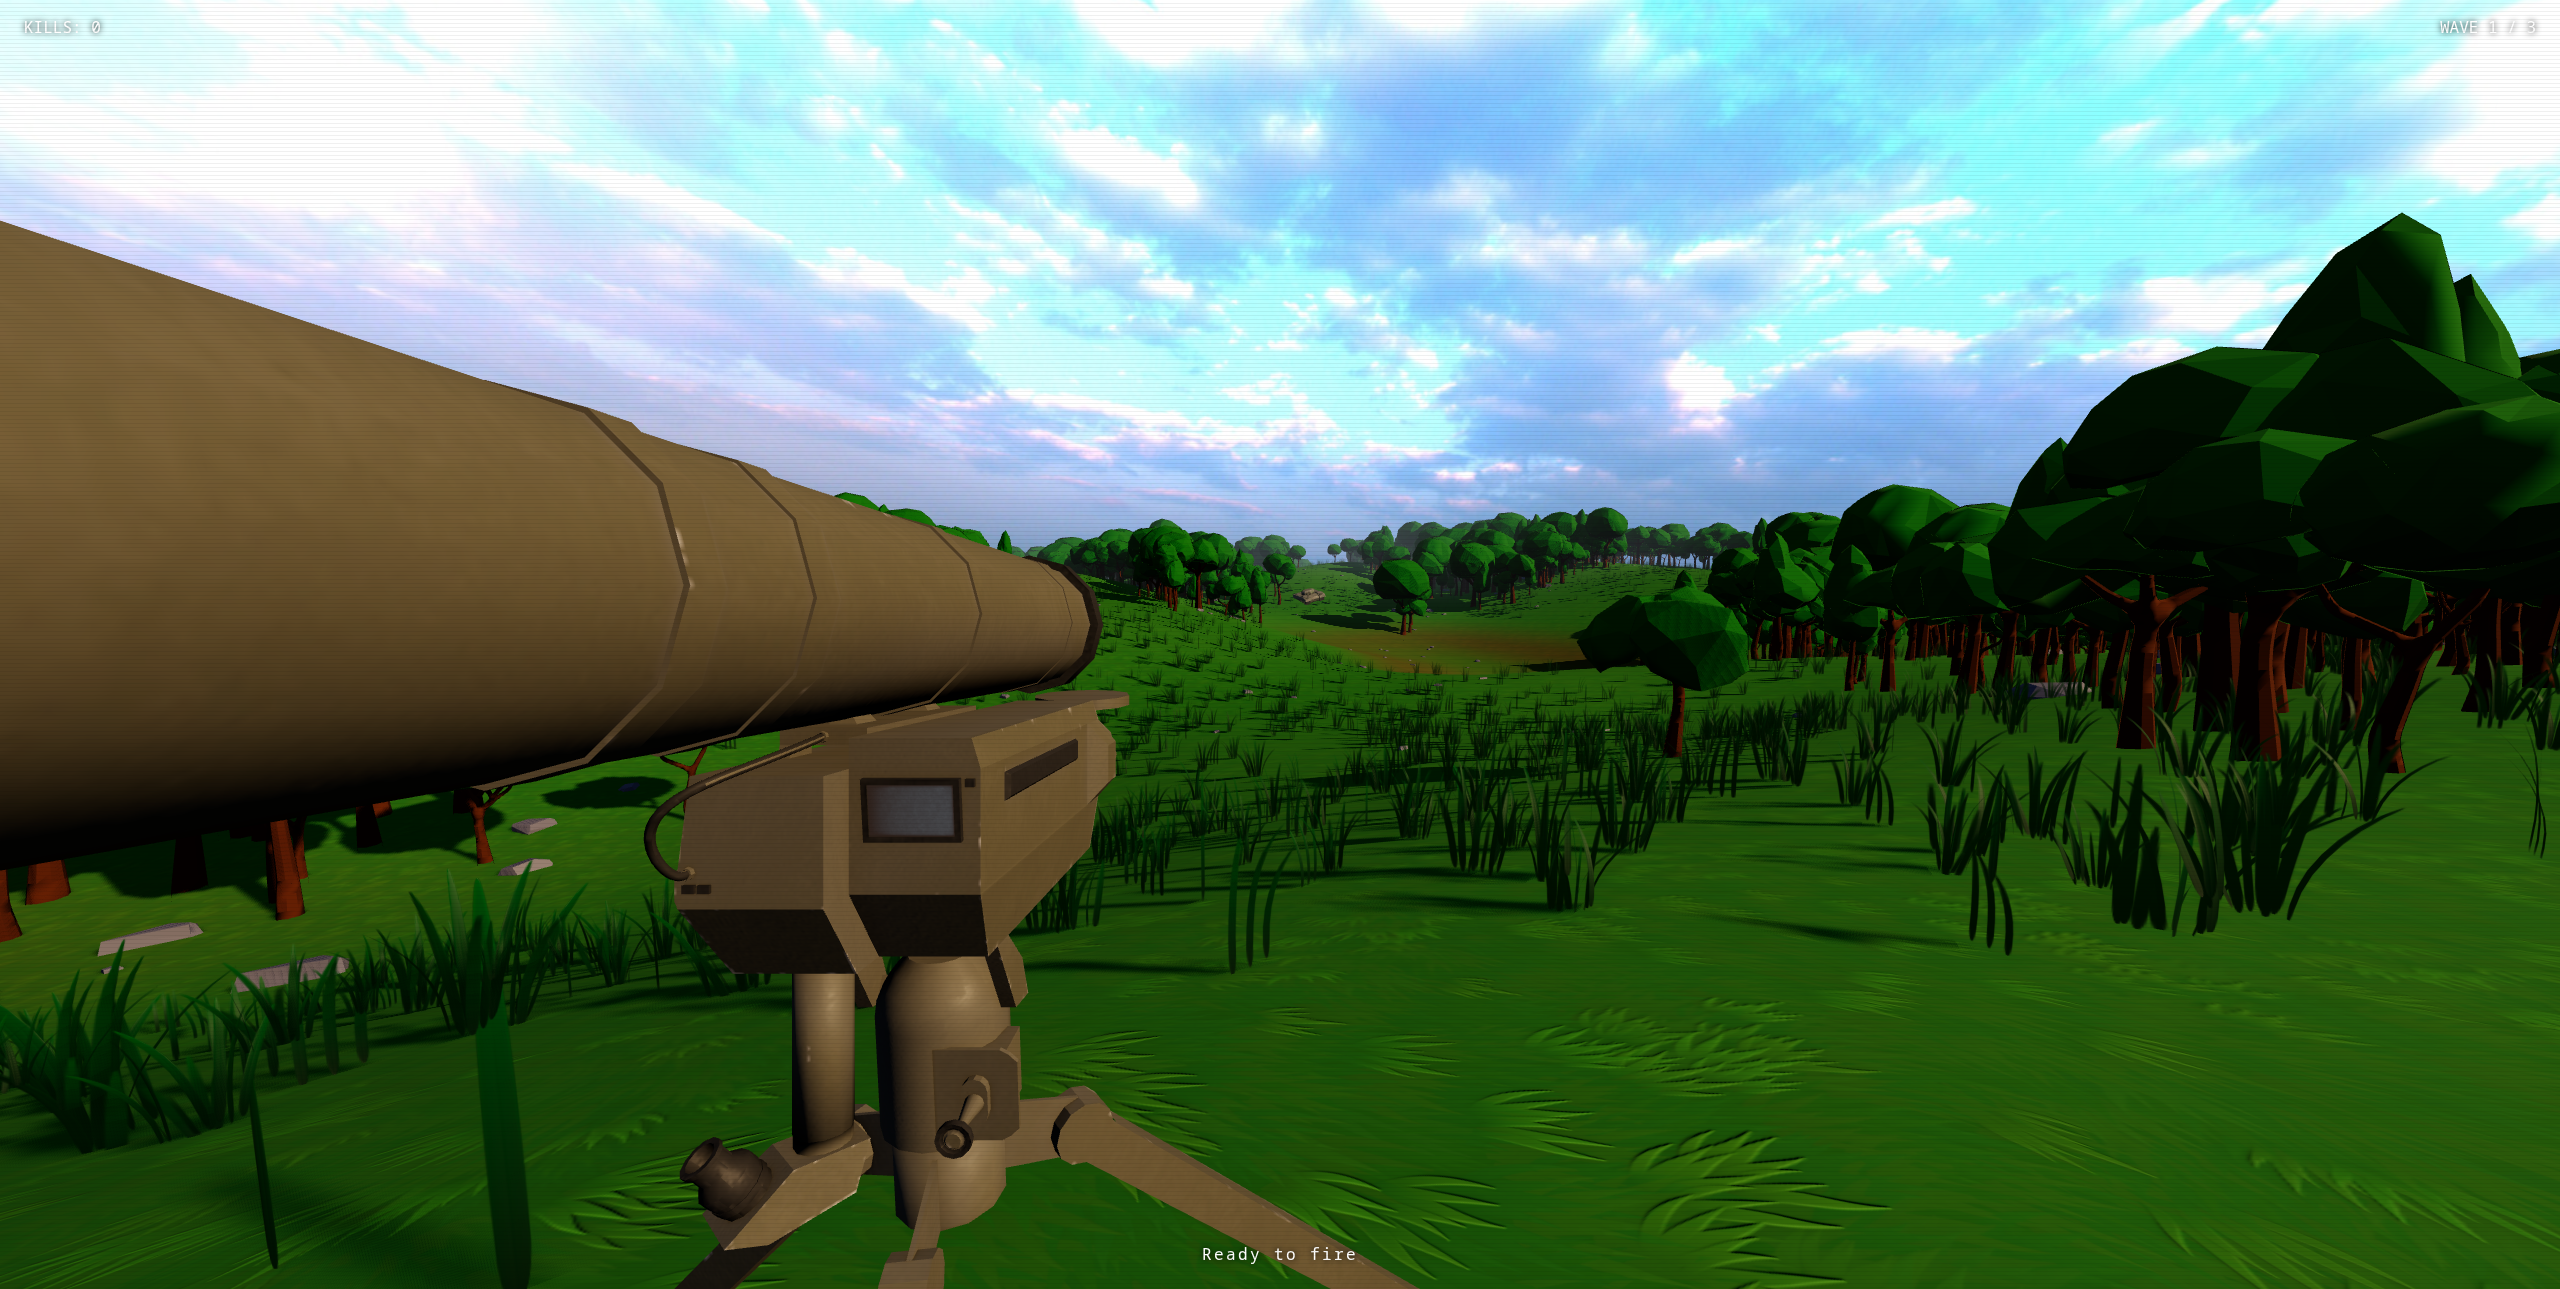
\includegraphics[width=\textwidth]{game.png}
		\caption{StaticDefense in play: enemy tanks advancing across procedurally generated terrain.}
		\label{fig:gameplay}
	\end{figure}

	% ════════════════════════════════════════════════════════════
	\section{Development Environment}

	\subsection{Rendering Library}

	The project uses \textbf{Three.js} (bundled via npm), a WebGL abstraction library with
	a native GLTF loader, PBR materials, and shadow mapping. No additional rendering
	library is used.

	\subsection{Build Tooling}

	\textbf{Vite} serves as the development server and module bundler. It provides ES-module
	native hot-module replacement during development and produces an optimized static bundle
	for deployment. The full source tree is listed below.

\begin{lstlisting}[language={}, caption={Project file tree}, label={lst:tree}]
StaticDefense/
|-- index.html               Scene selector / main entry point
|-- src/
|   |-- core/
|   |   |-- audio.js         Audio listener and sound loading helpers
|   |   |-- game.js          Wave definitions and win/lose logic
|   |   |-- navigation.js    A* pathfinding and nav grid
|   |   `-- terrain.js       Procedural terrain generation
|   |-- entities/
|   |   |-- clutter.js       Tree and rock placement (noise + tryBlock)
|   |   |-- grass.js         Billboard grass instancing
|   |   |-- launcher.js      Player launcher: bones, aiming, reload FSM
|   |   |-- missile.js       Guided missile: flight, collision, trail
|   |   |-- prop.js          Generic static prop loader
|   |   |-- tank.js          Enemy tank: AI, state machine, turret IK
|   |   `-- tv.js            TV intro prop and video texture
|   |-- rendering/
|   |   |-- effects.js       Particles, billboard fire and smoke
|   |   `-- materials.js     Shared PBR MeshStandardMaterials
|   |-- scenes/
|   |   |-- main.js          Main game scene
|   |   |-- intro.js         TV intro sequence
|   |   |-- menu_bg.js       Shared wireframe background (launcher spin)
|   |   |-- scene_loader.js  URL param router (?scene=X)
|   |   |-- debug_launcher.js  Isolated launcher + 6 tanks
|   |   |-- debug_model.js    Orbit viewer for all assets, wireframe 
|   |   |-- debug_tank.js     Single tank patrolling a fixed target
|   |   |-- debug_terrain.js  Live terrain sliders, navmap overlay toggle
|   |   `-- debug_tv.js       TV prop with video playback in isolation
|   |-- ui/
|   |   |-- hud.js           HUD elements and debug key legend
|   |   `-- transition.js    CSS fade-to-black overlay
|   `-- utilities/
|       `-- loader.js        GLTF loader wrappers
|-- public/
|   |-- models/              GLB files (launcher, tank, trees x4,
|   |                         grass x5, rocks x3, tv)
|   |-- textures/            Custom PBR texture sets per model, sky
|   |-- sounds/              OGG sound effects
|   |-- video/
|   |   `-- intro.mp4        TV intro video
|   `-- ui/
|       `-- crosshair.svg    Scope crosshair overlay
\end{lstlisting}

	\subsection{Deployment}

	The project is deployed via GitHub Pages from the repository root. The live demo is
	accessible at the URL listed on the title page.

	% ════════════════════════════════════════════════════════════
	\section{Libraries, Tools, and External Assets}

	\subsection{Third-Party Libraries}

	\begin{center}
		\begin{tabularx}{\textwidth}{llX}
			\toprule
			\textbf{Library} & \textbf{Version} & \textbf{Purpose} \\
			\midrule
			Three.js       & r165  & WebGL rendering, scene graph, materials, loaders \\
			Vite           & 5.x   & Development server and production bundler \\
			simplex-noise  & 4.0.3 & 2D simplex noise for terrain height and tree placement \\
			\bottomrule
		\end{tabularx}
	\end{center}

	\subsection{External Models}

	The following 3D models were sourced externally. The launcher model and all its textures
	were created entirely by the author in Blender. The tank mesh was downloaded from
	Sketchfab and edited; its textures were created from scratch.

	\begin{center}
		\begin{tabularx}{\textwidth}{llX}
			\toprule
			\textbf{Asset} & \textbf{Source} & \textbf{Notes} \\
			\midrule
			Launcher (9M133 Kornet) & Author (Blender) & Model and textures fully original \\
			Tank                    & Sketchfab (Kolos Studios) & Mesh edited; textures replaced \\
			Trees (4 variants)      & Sketchfab (SimplePolygon) & Used as-is \\
			Grass (5 variants)      & Sketchfab (Nicothin)      & Used as-is \\
			Rocks (3 variants)      & Sketchfab                 & Used as-is \\
			Television              & Sketchfab (mittelwerk)    & Used as-is \\
			\bottomrule
		\end{tabularx}
	\end{center}

	\subsection{Textures and Audio}

	The grass terrain PBR texture set was sourced from \textit{freestylized.com} (grass\_01),
	free for non-commercial use. Sky textures were sourced from \textit{Poly Haven}
	(public domain). Sound effects are royalty-free assets from \textit{Pixabay}, uploaded
	by user \textit{freesound\_community}. All other textures (launcher, tank, terrain) were
	authored by the project author.

	% ════════════════════════════════════════════════════════════
	\section{3D Assets}

	\subsection{9M133 Kornet Launcher}
	\label{sec:3dassets-launcher}

	The launcher is a fully original asset: geometry, UV unwrap, rig, and all PBR textures
	were created by the author from scratch in Blender using reference photographs of the
	real weapon system. Figure~\ref{fig:launcher} shows the in-game model alongside the
	reference image used during modelling.

	The skeleton was also rigged by the author in Blender. Five bones are exported as part
	of the GLTF file. \texttt{Base} is the static root; \texttt{Middle} and \texttt{Launcher}
	are the two aiming bones; \texttt{Tube} and \texttt{Sight} are both children of
	\texttt{Launcher}:

	\begin{center}
		\texttt{Base} $\to$ \texttt{Middle} $\to$ \texttt{Launcher}
		$\begin{cases} \to \texttt{Tube} \\ \to \texttt{Sight} \end{cases}$
	\end{center}

	All in-game animation (aiming, reloading, tube toss) drives these bones directly in
	JavaScript at runtime. No animation data is imported.

	\begin{figure}[h]
		\centering
		\begin{subfigure}[b]{0.48\textwidth}
			\centering
			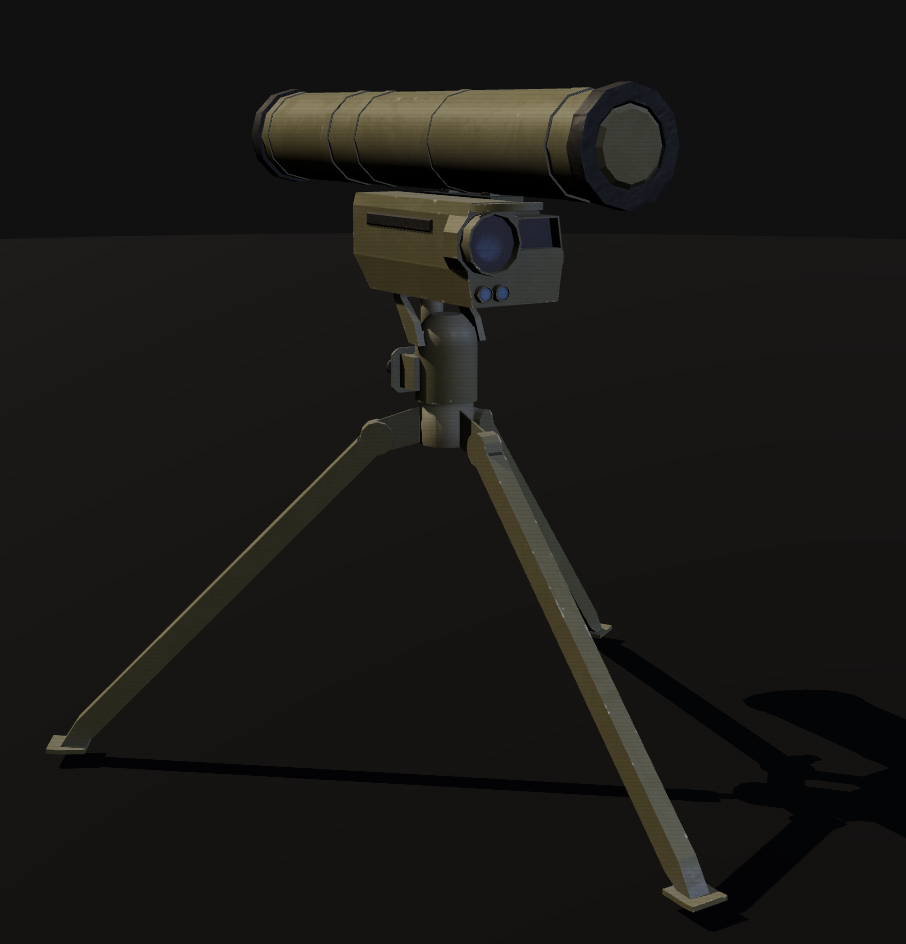
\includegraphics[width=\textwidth]{model.png}
			\caption{In-game 3D model}
		\end{subfigure}
		\hfill
		\begin{subfigure}[b]{0.48\textwidth}
			\centering
			\includegraphics[width=\textwidth]{real.png}
			\caption{Real 9M133 Kornet (reference)}
		\end{subfigure}
		\caption{The Kornet launcher: in-game model versus photographic reference.}
		\label{fig:launcher}
	\end{figure}

	\subsection{Enemy Tank}
	\label{sec:3dassets-tank}

	The tank mesh was downloaded from Sketchfab (Kolos Studios) and significantly edited in
	Blender to match the game's visual style and technical requirements. The skeleton was
	rigged entirely by the author: three bones (\texttt{Hull}, \texttt{Turret},
	\texttt{Gun}) drive the hull, rotating turret, and elevating gun respectively, making
	full turret IK tracking possible at runtime. All textures (base color, normal, AO,
	metalness, roughness) were created from scratch by the author. The design does not
	represent a specific vehicle but is loosely inspired by Soviet-era tank aesthetics.

	\begin{figure}[h]
		\centering
		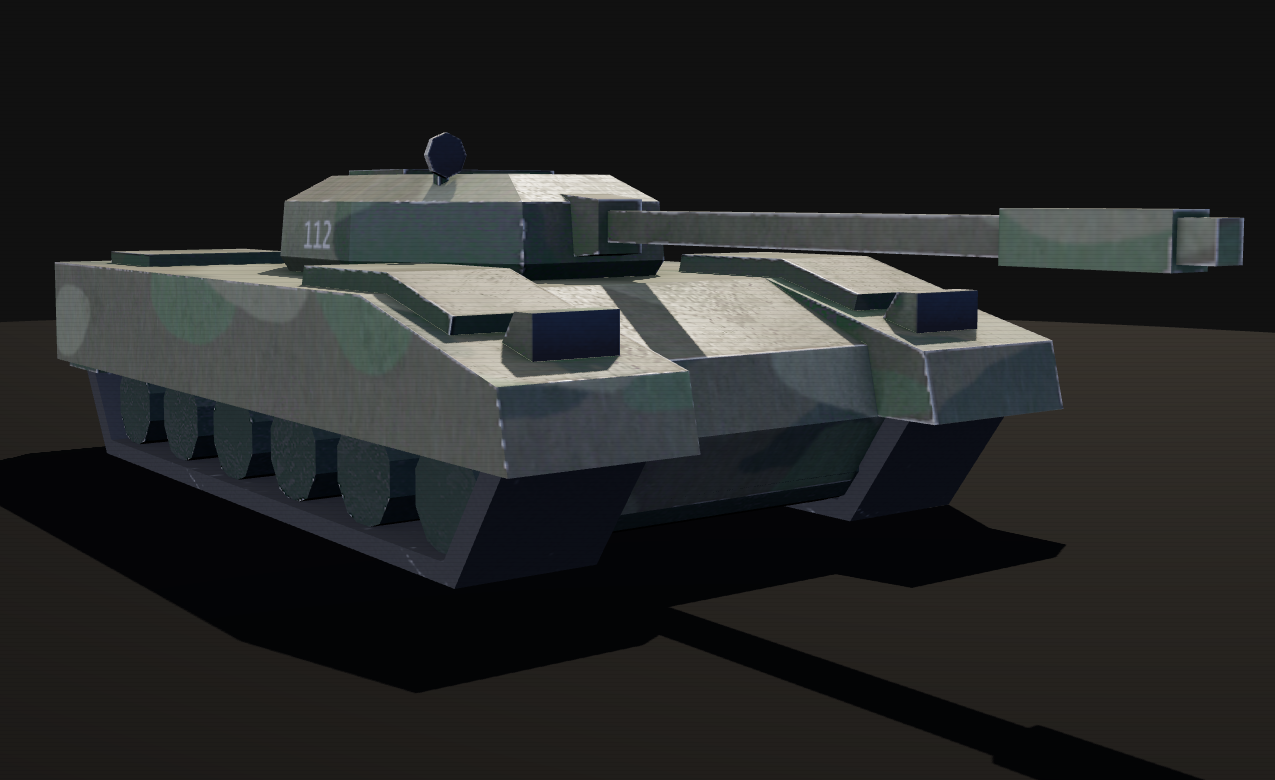
\includegraphics[width=0.82\textwidth]{tank.png}
		\caption{The enemy tank with custom PBR textures and three-bone rig.}
		\label{fig:tank}
	\end{figure}

	% ════════════════════════════════════════════════════════════
	\section{Technical Description}

	\subsection{Hierarchical Models}

	Both models are rigged in Blender and driven entirely in JavaScript at runtime; no
	animation data is imported.

	\subsubsection{9M133 Kornet Launcher}

	The five-bone skeleton is described in Section~\ref{sec:3dassets-launcher}. At runtime,
	mouse input drives \texttt{Middle} (azimuth) and \texttt{Launcher} (elevation pitch)
	directly each frame. Because the scene graph hierarchy is exploited, a single rotation
	on \texttt{Middle} automatically carries \texttt{Launcher}, \texttt{Tube}, and
	\texttt{Sight} with no manual matrix decomposition.

	The reload sequence drives \texttt{Tube} through five states, all coded in JavaScript:

	\begin{center}
		\texttt{READY} $\to$ \texttt{FIRED} $\to$ \texttt{POST\_FIRE} $\to$
		\texttt{TOSSING} $\to$ \texttt{RELOADING} $\to$ \texttt{READY}
	\end{center}

	In \texttt{TOSSING}, the tube mesh is detached from the bone, given a world-space
	velocity, and arcs to the terrain under simulated gravity. The \texttt{Sight} bone
	projects the scope camera direction into world space each frame to compute the firing
	ray.

	\subsubsection{Enemy Tank}
	\label{sec:tech-tank}

	The tank's three-bone hierarchy (\texttt{Hull} $\to$ \texttt{Turret} $\to$ \texttt{Gun})
	is described in Section~\ref{sec:3dassets-tank}. At runtime the turret yaw and gun pitch
	are solved analytically each frame to track the launcher position, accounting for the
	rest-pose offset baked in Blender. Because \texttt{Gun} is a child of \texttt{Turret},
	the gun automatically inherits the turret's world rotation; only the relative elevation
	angle needs to be set. Invisible proxy boxes are parented to each bone so missile
	raycasting tracks the animated skeleton.

	\subsection{Procedural Terrain}

	\begin{figure}[h]
		\centering
		\begin{tcolorbox}[pipelinebox]
			\centering
			\begin{tabular}{c}
				\textbf{Constructor init} \\
				{\small PlaneGeometry, noise maps, NavigationMap} \\[4pt]
				$\downarrow$ \\[4pt]
				\multicolumn{1}{c}{\textit{\small $\hookleftarrow$\ retry loop (max 10 attempts)}} \\[4pt]
				$\downarrow$ \\[4pt]
				\texttt{generateHeights()} \quad {\small two-octave simplex noise, quantised to discrete steps} \\
				$\downarrow$ \\
				\texttt{applyVertexColors()} \quad {\small dirt / grass / rock blended by height and slope} \\
				$\downarrow$ \\
				\texttt{computeVertexNormals()} \\
				$\downarrow$ \\
				\texttt{blockSteepCells()} \quad {\small mark impassable nav-grid cells} \\
				$\downarrow$ \\
				Snap enemy spawn positions to terrain Y \\
				$\downarrow$ \\
				\texttt{findSuitableLauncherSpawn()} \quad {\small score 120 candidates} \\
				$\downarrow$ \\
				\textbf{launcher.y $\geq$ MIN\_HEIGHT?} \\
				{\small No $\longrightarrow$ re-seed noise, repeat loop} \\
				{\small Yes $\downarrow$} \\[4pt]
				Hill boost around launcher spawn \quad {\small radius 40\,u, up to $+3$\,u} \\
				$\downarrow$ \\
				\texttt{computeProtectedCells()} \quad {\small A* corridors from every enemy spawn} \\
				$\downarrow$ \\
				\textbf{Terrain ready}
			\end{tabular}
		\end{tcolorbox}
		\caption{Terrain generation pipeline. The retry loop re-seeds the noise until the
			launcher candidate clears the minimum height threshold, ensuring it always sits
			on a visible rise.}
		\label{fig:terrain-pipeline}
	\end{figure}

	Vertex colors are computed per-vertex from two factors: a normalized height value
	$h \in [0,1]$ and a slope value derived from the dot product of the vertex normal with
	the world up vector. Low elevations blend toward brown (dirt), mid-range heights toward
	green (grass), and steep faces toward grey (rock). Flat areas receive a flatness bonus
	that forces them toward grass regardless of absolute height, preventing plains from
	reading as dirt.

	The launcher spawn scoring weighs four criteria: absolute elevation, local terrain
	flatness, distance from enemy spawn positions, and estimated line-of-sight exposure
	toward all enemy approach corridors. The best-scoring candidate from 120 sampled
	positions is selected.

	\begin{figure}[h]
		\centering
		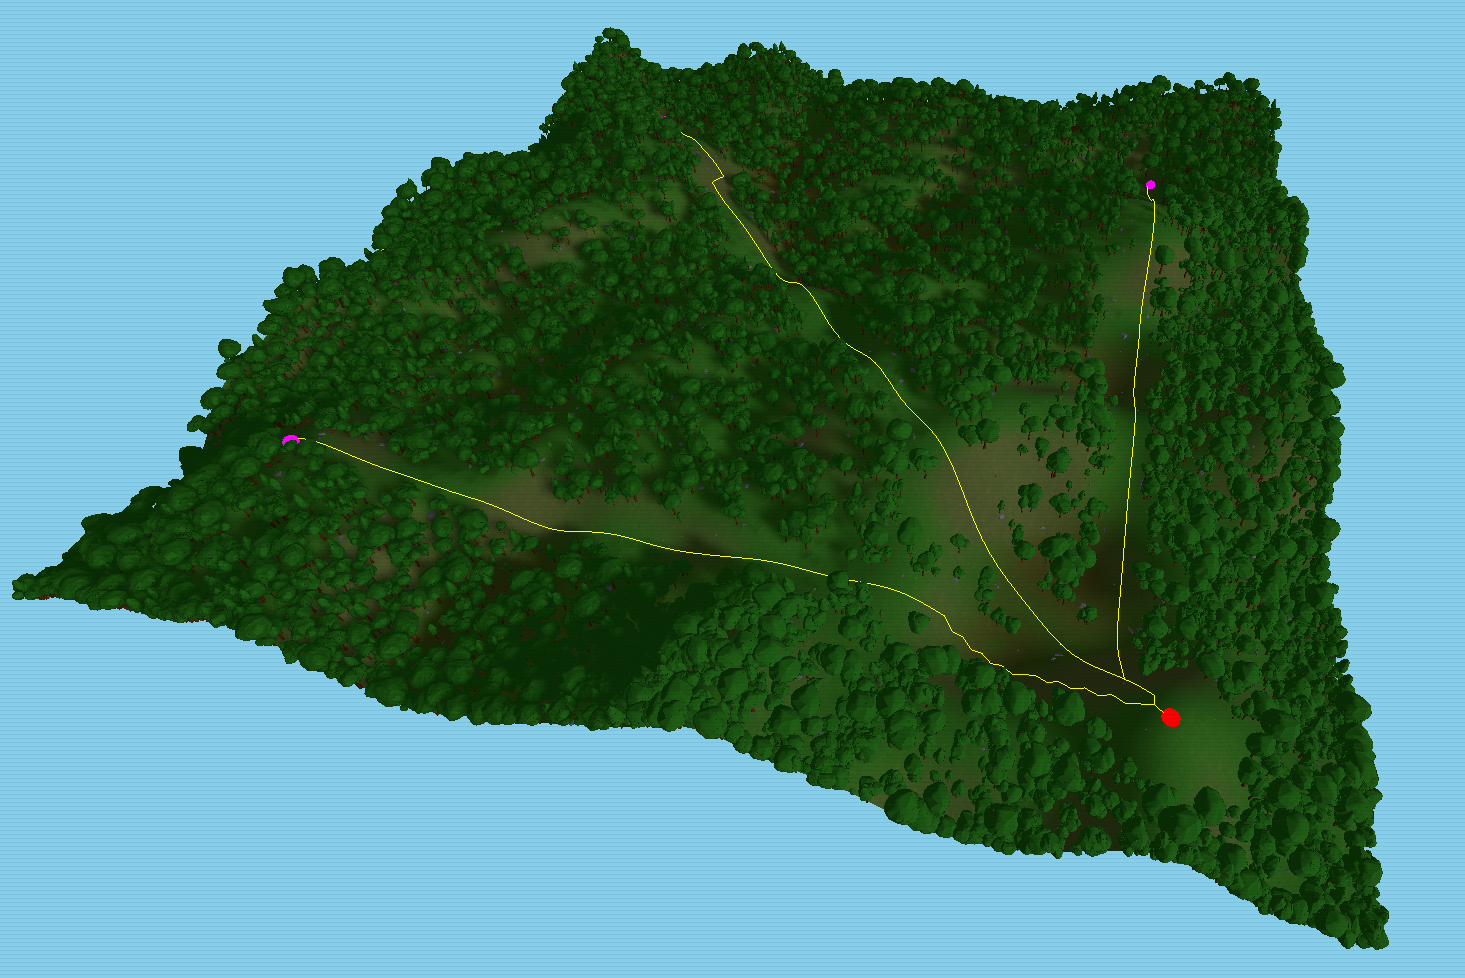
\includegraphics[width=\textwidth]{terrain.png}
		\caption{A generated terrain showing height-based vertex color blending, clutter
			placement, and the launcher hill boost near the center-right.}
		\label{fig:terrain}
	\end{figure}

	\subsection{Navigation and Pathfinding}

	A grid-based A* implementation in \texttt{src/core/navigation.js} handles all tank
	movement. The grid covers the terrain at a fixed cell resolution. Each cell is marked
	passable or impassable based on terrain slope and the presence of large rocks.

	The search explores all 8 neighbors (4 cardinal + 4 diagonal). Diagonal moves are
	assigned cost $\sqrt{2}$ and are rejected if either adjacent cardinal cell is blocked,
	preventing tanks from squeezing through tight diagonal gaps.

	At startup, a path is computed from every enemy spawn to the launcher position, and a
	buffer of cells around each path is stored as \textit{protected corridors}. Clutter
	placement respects these corridors: when a large rock candidate falls inside one, it is
	tentatively placed and a BFS connectivity check is run from the launcher. If any spawn
	becomes unreachable, the rock is removed. This allows rocks to appear inside corridors
	without ever fully blocking the AI.

	If a tank does not advance meaningfully for 1.5 seconds (stuck on geometry), it
	immediately re-plans from its current position.

	\begin{figure}[h]
		\centering
		\begin{subfigure}[b]{0.48\textwidth}
			\centering
			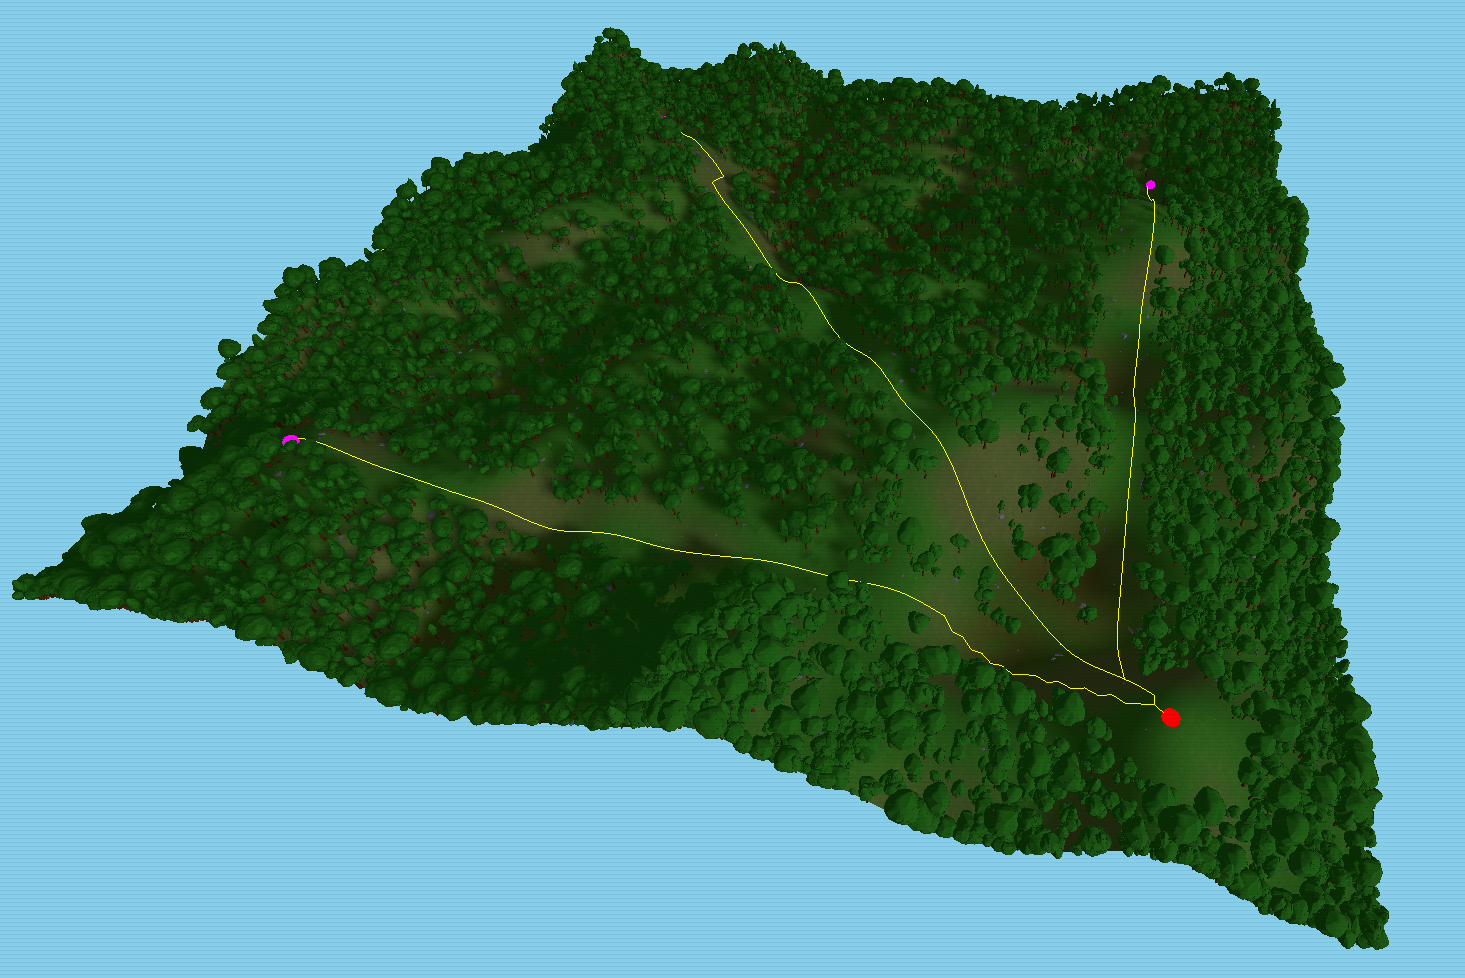
\includegraphics[width=\textwidth]{terrain.png}
			\caption{Generated terrain with vertex colors, trees, clutter and paths.}
		\end{subfigure}
		\hfill
		\begin{subfigure}[b]{0.48\textwidth}
			\centering
			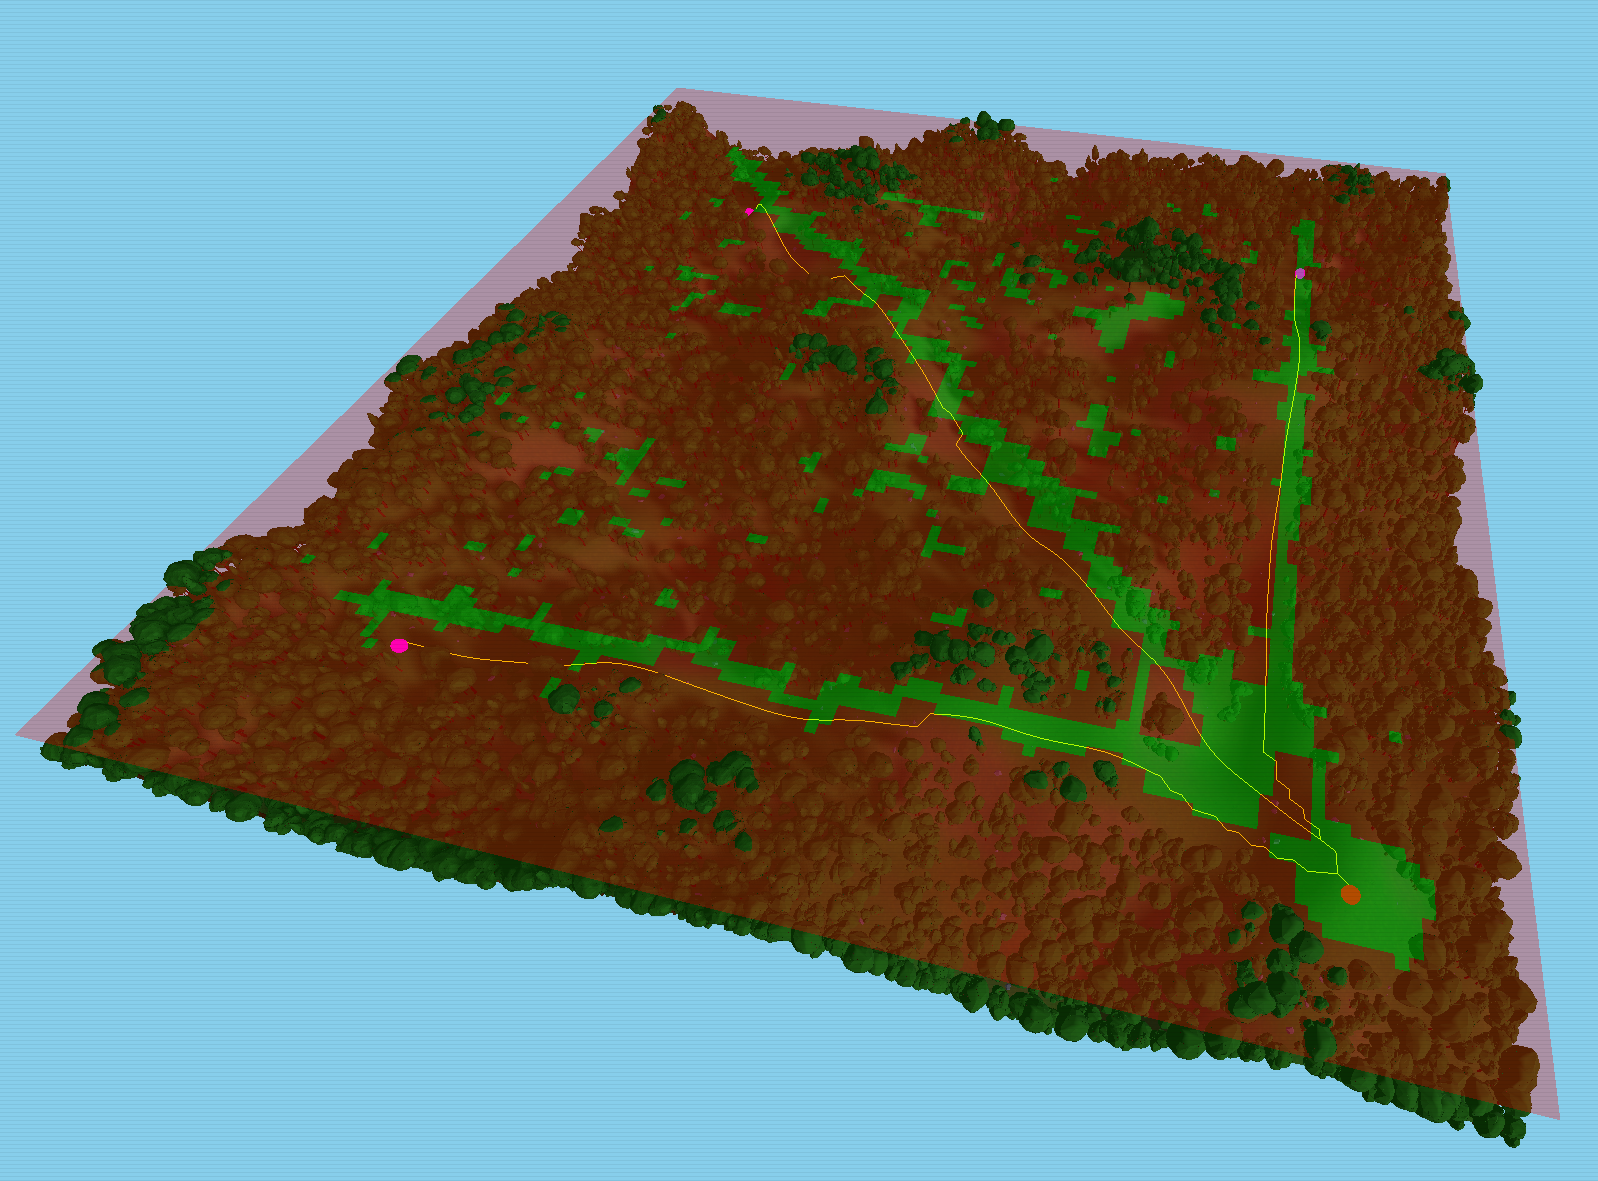
\includegraphics[width=\textwidth]{navmap.png}
			\caption{A* nav grid overlay (green: passable, red: blocked)}
		\end{subfigure}
		\caption{The same map shown with and without the navigation grid overlay,
			visible in the \texttt{debug\_terrain} scene.}
		\label{fig:navmap}
	\end{figure}

	\subsection{Tank AI}

	Each tank is a state machine with four states:

	\begin{center}
		\begin{tabular}{ll}
			\toprule
			\textbf{State} & \textbf{Behaviour} \\
			\midrule
			\texttt{ALIVE}   & Following A* path, turret tracking launcher \\
			\texttt{HIT}     & Speed reduced, hull fire started \\
			\texttt{COOKOFF} & Stopped, turret fire, secondary explosions \\
			\texttt{DEAD}    & Static charred wreck, nav cell blocked \\
			\bottomrule
		\end{tabular}
	\end{center}

	Turret aiming is covered in Section~\ref{sec:tech-tank}: yaw and pitch are solved analytically each
	frame, accounting for the 90\textdegree{} rest-pose offset baked in Blender.

	When a tank is assigned its path, its destination is offset by a random $\pm$8 world
	units on X and Z, so tanks from the same spawn point don't march in a single column.

	Tanks also conform to terrain slope: two height samples are taken along the forward and
	side axes each frame, and the pitch and roll are set to match the local terrain normal.
	On death, the material is cloned and tinted dark (\texttt{0x1a1a1a}) with a faint
	emissive glow, keeping the shared base material intact across all living tanks.

	\subsection{Missile System}

	After launch, the missile is updated each frame by the guidance loop:

	\begin{enumerate}[itemsep=3pt]
		\item The missile's current forward direction is linearly interpolated toward the
		      vector from the missile position to the player's aim reticle (MCLOS guidance).
		\item The new direction is normalized and the missile is translated by
		      \texttt{speed * delta}.
		\item A ray is cast from the previous position to the current position against all
		      world meshes (terrain, rocks, tree trunks). The first intersection triggers an
		      impact explosion.
		\item Tanks expose invisible proxy box meshes parented to the hull, turret, and gun
		      bones. The missile raycasts against this proxy group to register hits on the
		      animated skeleton.
		\item The missile self-destructs after travelling 550 world units.
	\end{enumerate}

	A particle fire trail is emitted at fixed time intervals behind the missile. Each
	particle is given a randomized outward velocity with upward bias and scales to zero over
	its lifetime; gravity is applied per-frame.

	\subsection{Lighting and Textures}

	The main scene uses two light sources:

	\begin{itemize}[itemsep=3pt]
		\item \textbf{Directional light} (sun): warm color \texttt{0xffd6a3}, positioned
		      to suggest afternoon light. PCF shadow mapping at 2048$\times$2048 resolution,
		      with a \texttt{shadowBias} of \texttt{-0.0005} to suppress surface acne.
		\item \textbf{Ambient light}: very low intensity (0.05) fill to prevent fully
		      black shadow regions.
	\end{itemize}

	The launcher and tank both use \texttt{MeshStandardMaterial} with the following
	texture maps:

	\begin{center}
		\begin{tabular}{ll}
			\toprule
			\textbf{Map} & \textbf{Applied to} \\
			\midrule
			Albedo (base color) & Launcher, tank, terrain \\
			Normal map          & Launcher, tank, terrain \\
			Ambient occlusion   & Launcher, tank, terrain \\
			Metalness map       & Launcher, tank \\
			Roughness map       & Launcher, tank \\
			Video texture       & TV intro screen (MP4) \\
			\bottomrule
		\end{tabular}
	\end{center}

	Terrain uses a PBR texture set with repeat tiling ($50\times50$) across the mesh, plus
	per-vertex color blending to produce the height/slope-dependent dirt-grass-rock
	appearance described in the Procedural Terrain section above.

	ACES filmic tone mapping is enabled on the renderer.

	\subsection{Environment and Rendering Effects}

	\subsubsection{Scope view}
	When the player toggles the scope (right mouse button), a radial-gradient CSS overlay
	is added over the canvas: transparent in the center, nearly opaque at the edges,
	producing a rifle-scope vignette. A second full-screen canvas of resolution
	$320\times180$ (scaled up) is placed below the vignette and updated every frame with
	sparse random bright pixels over a very-low-level grey noise. The blend mode
	\texttt{mix-blend-mode:~screen} makes it read as a digital CCTV grain visible only
	through the scope.

	\subsubsection{Particle explosions}
	Impact explosions spawn a burst of spherical particles with randomized outward velocity,
	slightly biased upward. Each particle scales to zero over its lifetime while gravity
	pulls it down.

	\subsubsection{Billboard fire and smoke}
	Two separate sprite systems are attached to damaged tanks: hull fire activates on
	\texttt{HIT} and turret fire on \texttt{COOKOFF}. Each sprite is a camera-facing plane
	that rises, fades, and resets in a loop. Hull and turret systems run concurrently during
	cookoff.

	\subsubsection{Environment clutter and GPU instancing}
	Trees, rocks, and grass use \texttt{THREE.InstancedMesh} to keep draw calls flat as
	clutter density scales up. Each geometry variant gets one instanced mesh; placement
	writes a transform matrix per instance rather than spawning individual scene objects.

	Trees are placed using dual-layer simplex noise (a cluster pass and a detail pass) to
	group them into clusters. Density is biased higher near map boundaries so the terrain
	edge does not read as a hard wall. Each placed tree also gets an invisible cylinder
	proxy (radius 0.75\,u, height 5\,u) for missile raycasting.

	Grass is placed in clusters: \texttt{density} $\times$ 60 cluster centers are chosen
	uniformly, then 20 blades are scattered around each center using polar coordinates with
	a square-root radius distribution (ensuring uniform disk coverage). Blades on slopes
	steeper than 0.45 or at low elevations (bare dirt) are skipped, so grass only appears
	where the vertex colors are green. Each variant gets a flat green tint
	(\texttt{0x00A728}) with a faint emissive component so it reads clearly in shadow.

	Large rocks are aligned to terrain normals via finite-difference slope sampling and
	generate collision proxies for missile raycasting. A second pebble pass
	($\approx\frac{1}{3}$ scale) scatters freely without nav or collision impact.

	\subsubsection{Sky and fog}
	The sky is an equirectangular JPEG mapped as a scene background. Linear fog
	(\texttt{THREE.Fog}) blends the scene to a grey-blue that matches the horizon, so the
	terrain boundary fades out rather than cutting off.

	\subsection{Audio}

	All in-game sounds use Three.js \texttt{PositionalAudio} attached to their source
	objects, so volume and stereo panning respond automatically to camera position and
	orientation via the Web Audio API.

	Sound events include: tank engine loop, track rattle, turret rotation, tank explosion,
	missile launch, missile impact, tube toss, tube drop, and reload click.

	Engine volume ramps smoothly via \texttt{linearRampToValueAtTime} when tanks start
	or stop, avoiding audible clicks. The reload sequence is split into two audio cues:
	the drop sound triggers the moment the spent tube nears the ground (before visual
	contact), and the reload click fires when the fresh round locks in, keeping audio
	and animation tightly synchronized.

	\subsection{Intro Sequence and Transitions}

	If the intro is enabled in the pre-game menu, a separate Three.js scene renders a 3D
	pocket television playing a looping video texture. The player can skip it with Enter. A CSS-animated
	fade-to-black overlay handles the transition into and out of the intro and between
	scene changes.

	The video itself was edited by the author in Adobe Premiere, cutting together old
	advertisements and telefilm footage found online with a clip from a Brezhnev speech,
	to give the intro a Soviet-era broadcast feel.

	\begin{figure}[h]
		\centering
		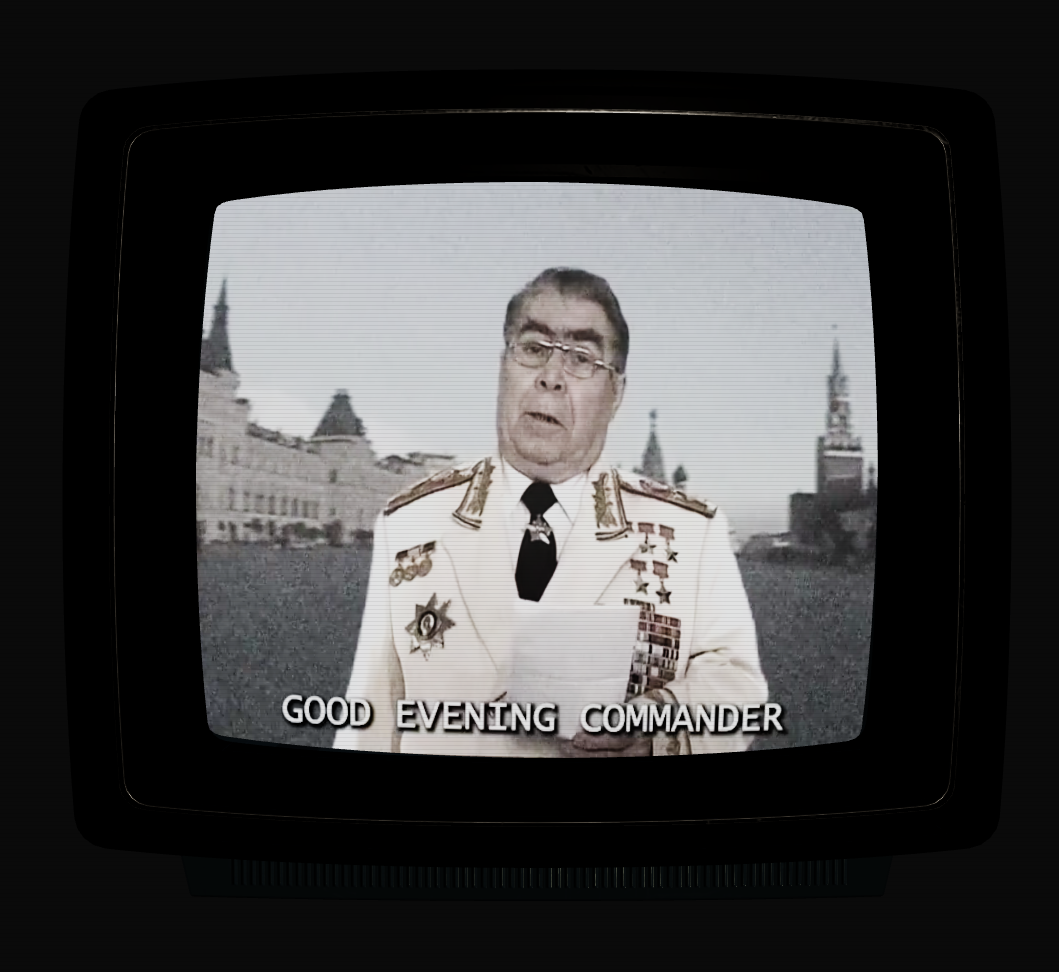
\includegraphics[width=\textwidth]{tv.png}
		\caption{The intro sequence: a 3D pocket television playing the edited video texture.}
		\label{fig:tv}
	\end{figure}

	The scene selector (\texttt{index.html}) renders a spinning wireframe of the launcher
	model in its left panel background, using a dedicated \texttt{WebGLRenderer} on a
	secondary canvas so it does not conflict with the main game renderer.

	% ════════════════════════════════════════════════════════════
	\section{User Interaction}

	\subsection{Pre-Game Setup}
	
	\begin{figure}[h]
		\centering
		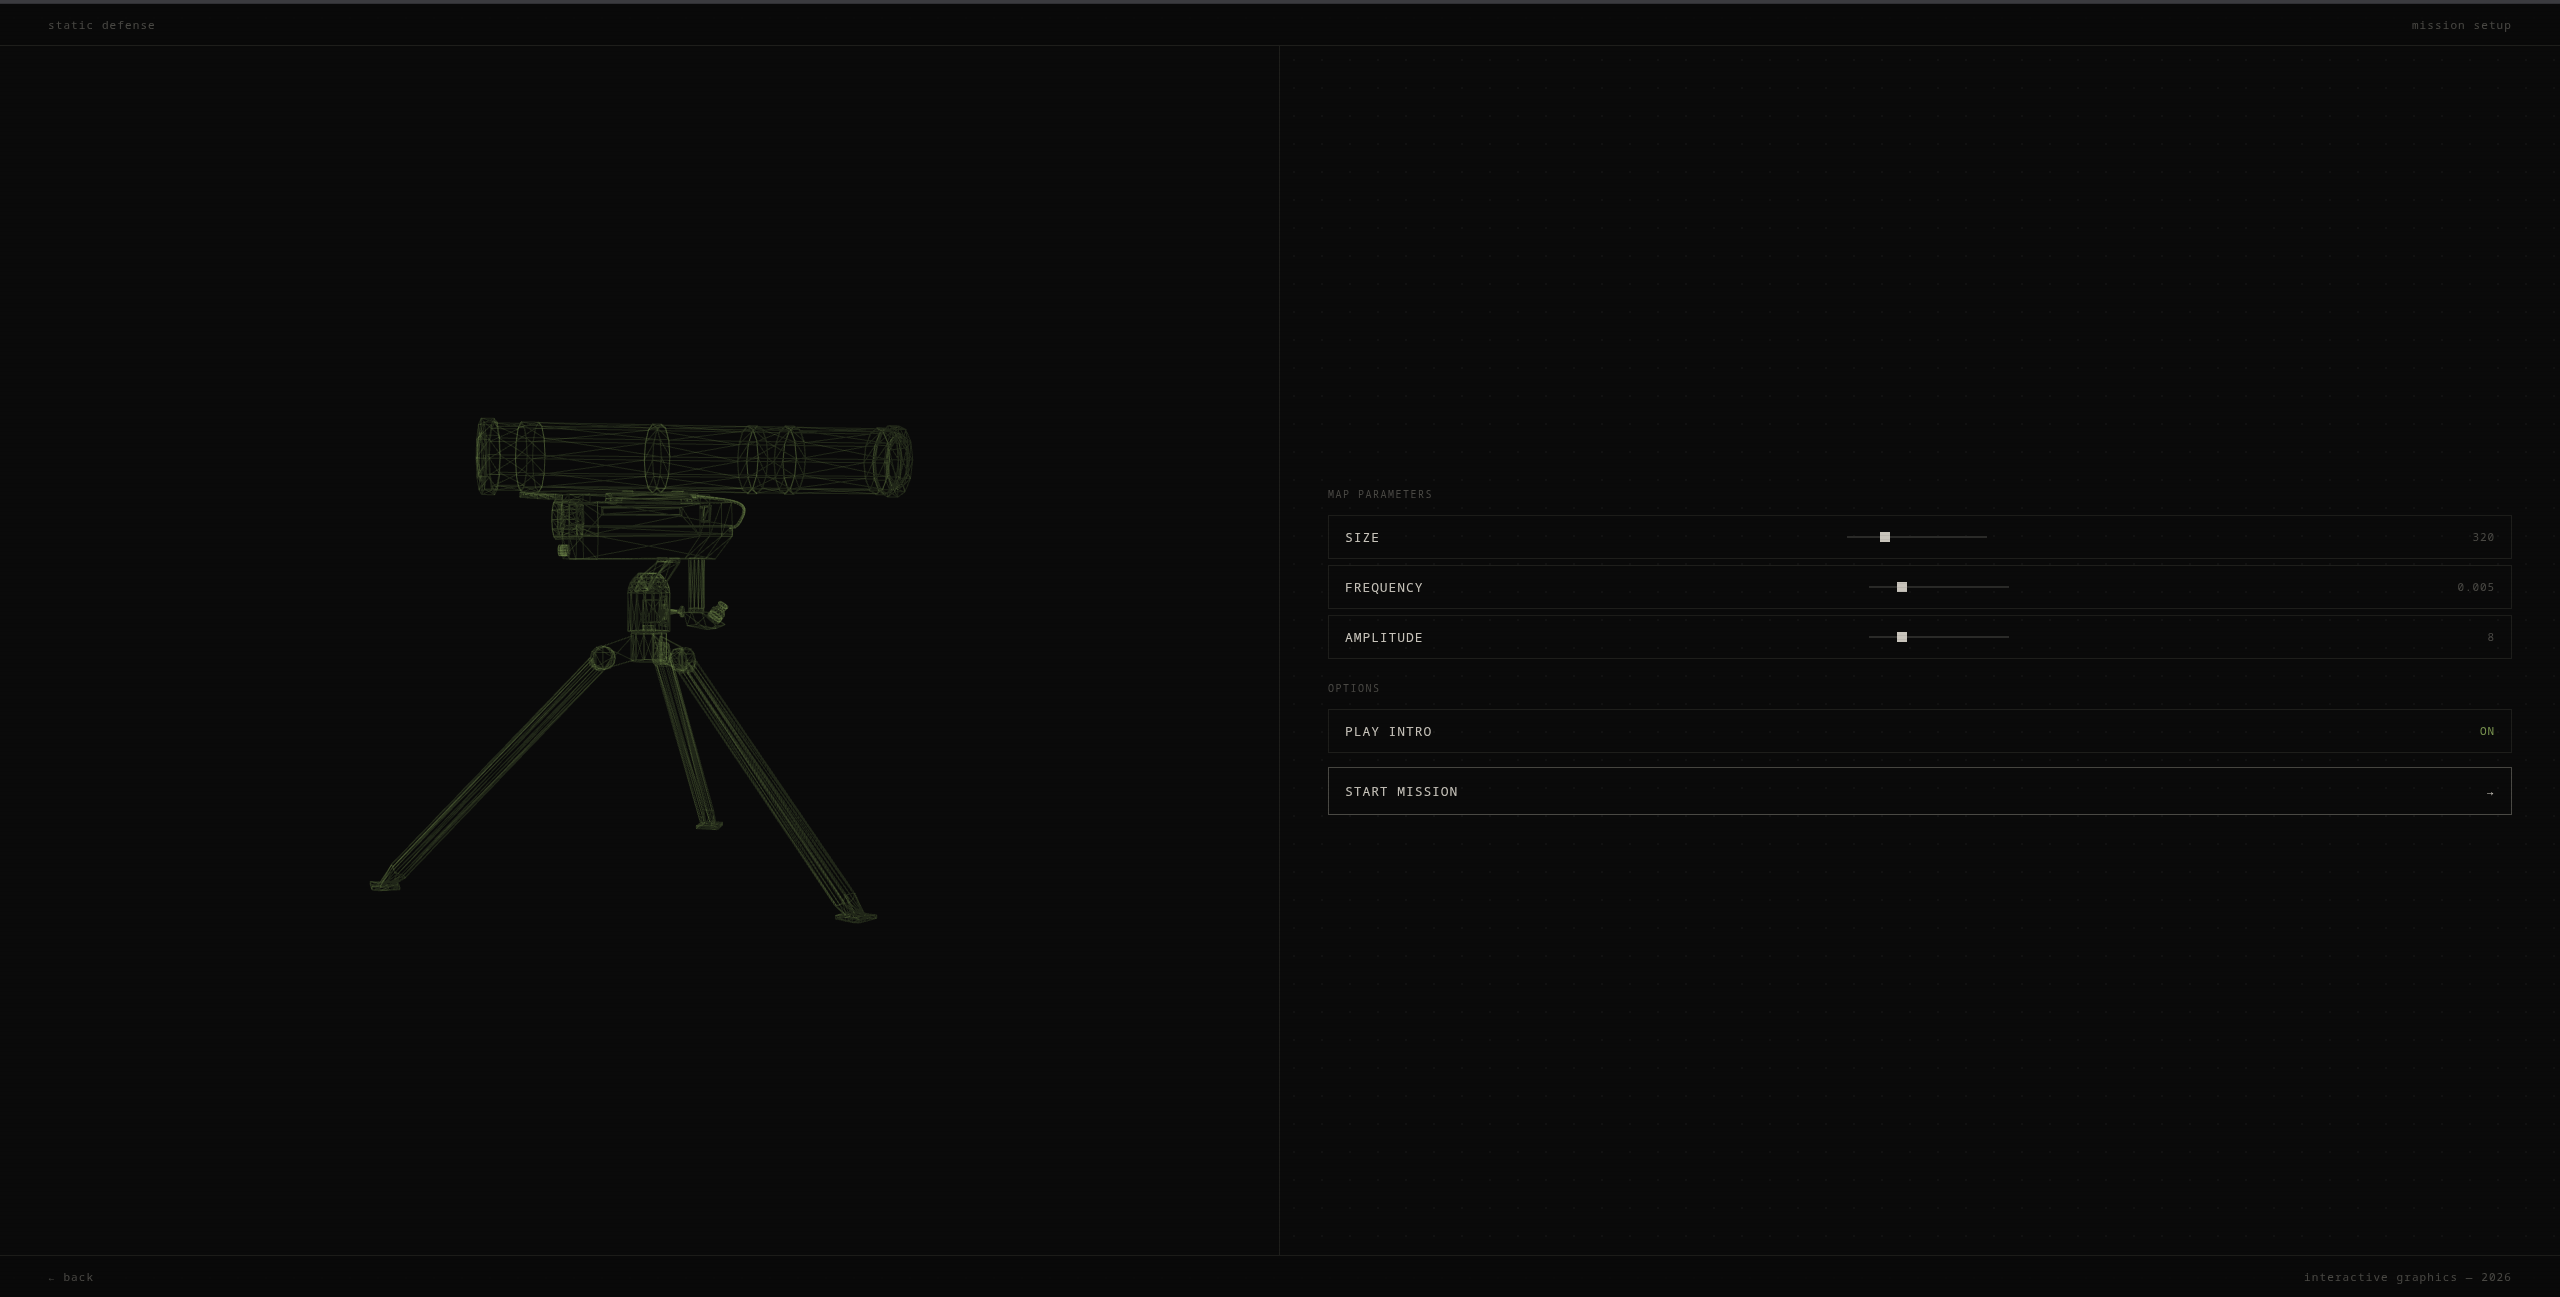
\includegraphics[width=\textwidth]{innermenu.png}
		\caption{Pre-game menu and its settings.}
		\label{fig:pre-game menu}
	\end{figure}

	Before the game loads, a full-screen menu lets the player configure the run. Three
	sliders adjust the terrain generation parameters: \textbf{size} (map extent),
	\textbf{frequency} (noise scale, controls hill density), and \textbf{amplitude}
	(maximum terrain height). A toggle selects whether the TV intro plays before the
	game begins. A \textit{Play} button loads the game scene with the chosen settings;
	a \textit{Back} button returns to the scene selector.

	\subsection{Gameplay Flow}

	On load, a TV intro scene plays a video texture on a 3D pocket television.
	The player skips it with Enter. The game scene fades in with a wave announcement.
	The player clicks to lock the pointer, then uses the mouse to rotate and elevate the
	launcher. Right-clicking toggles the scope vignette, which enables firing. After a
	hit or miss the player presses \texttt{R} to reload, watching the tube-toss animation
	before the next shot is ready. Three waves of increasing tank count must be cleared to
	win.

	\subsection{In-Game Controls}

	\begin{center}
		\begin{tabularx}{\textwidth}{llX}
			\toprule
			\textbf{Input} & \textbf{Context} & \textbf{Effect} \\
			\midrule
			Mouse move          & Always      & Rotates and pitches the launcher \\
			Left click          & Unfocused   & Lock pointer (required for mouse aim) \\
			Right click         & Always      & Toggle scope / sniper view \\
			Left click          & Scoped only & Fire guided missile \\
			\texttt{R}          & Post-fire   & Begin manual reload sequence \\
			\texttt{← →}       & Always      & Rotate launcher (keyboard alternative) \\
			\texttt{↑ ↓}       & Always      & Elevate launcher (keyboard alternative) \\
			\texttt{Enter}      & TV intro    & Skip intro sequence \\
			\bottomrule
		\end{tabularx}
	\end{center}

	Aiming is only possible with the pointer locked. Firing is only possible while scoped.
	The reload key is only accepted in the \texttt{POST\_FIRE} state; pressing it earlier
	has no effect.

	% ════════════════════════════════════════════════════════════
	\section{Game Logic}

	\subsection{Wave System}

	Three waves of increasing size are hard-coded in \texttt{src/core/game.js} as a
	\texttt{WAVE\_DEFINITIONS} array. Wave 1 spawns 2 tanks, wave 2 spawns 3, and wave 3 spawns 4. Each wave specifies the indices
	of the enemy spawn positions to use, distributing tanks around the map perimeter.

	The next wave does not begin until every tank from the current wave is in the
	\texttt{DEAD} state, giving the player time to reload before the next wave starts. A center-screen announcement fades in and out over 2 seconds on
	each wave start.

	\subsection{Win and Lose Conditions}

	\begin{itemize}[itemsep=3pt]
		\item \textbf{Win}: all tanks across all three waves are destroyed. An end screen
		      appears with the text \texttt{POSITION HELD}.
		\item \textbf{Lose}: any tank reaches the launcher position (within a threshold
		      distance). The end screen shows \texttt{DEFENSE FAILURE}.
	\end{itemize}

	The end screen is a DOM overlay with corner brackets, scanlines, and a typewriter
	title animation. On the lose screen, the title text periodically glitches with a
	CSS character-replacement effect.

	\begin{figure}[h]
		\centering
		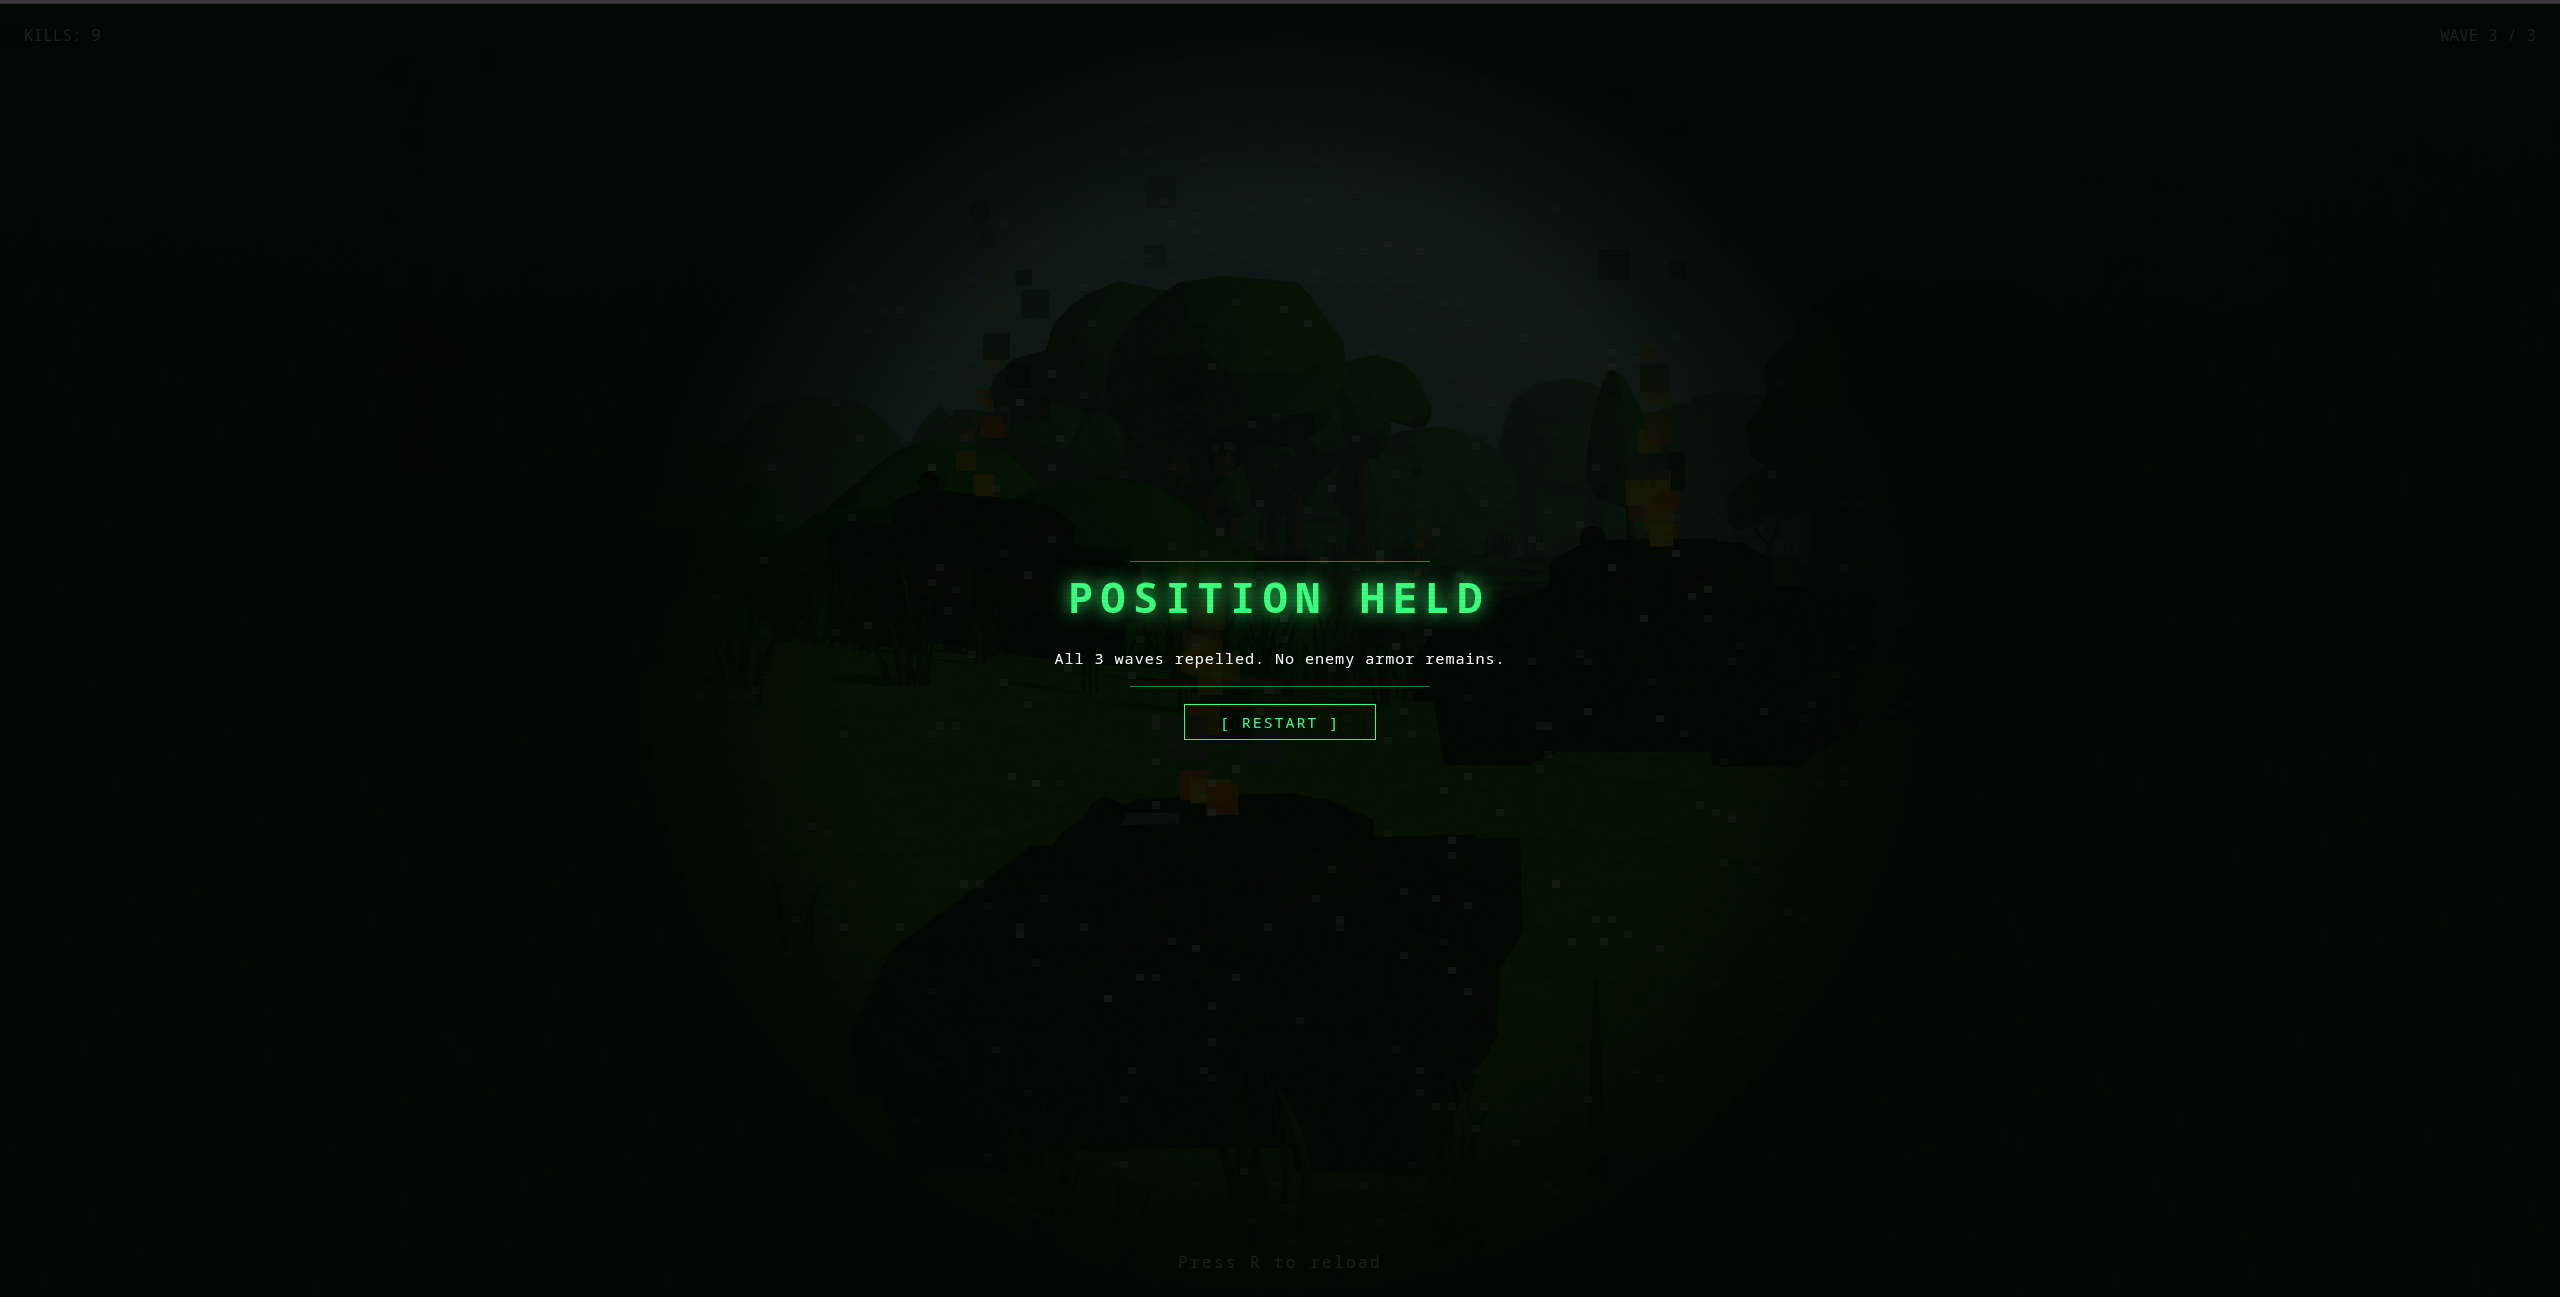
\includegraphics[width=\textwidth]{win.png}
		\caption{Victory screen after defeating all tanks.}
		\label{fig:win-screen}
	\end{figure}

	\begin{figure}[h]
		\centering
		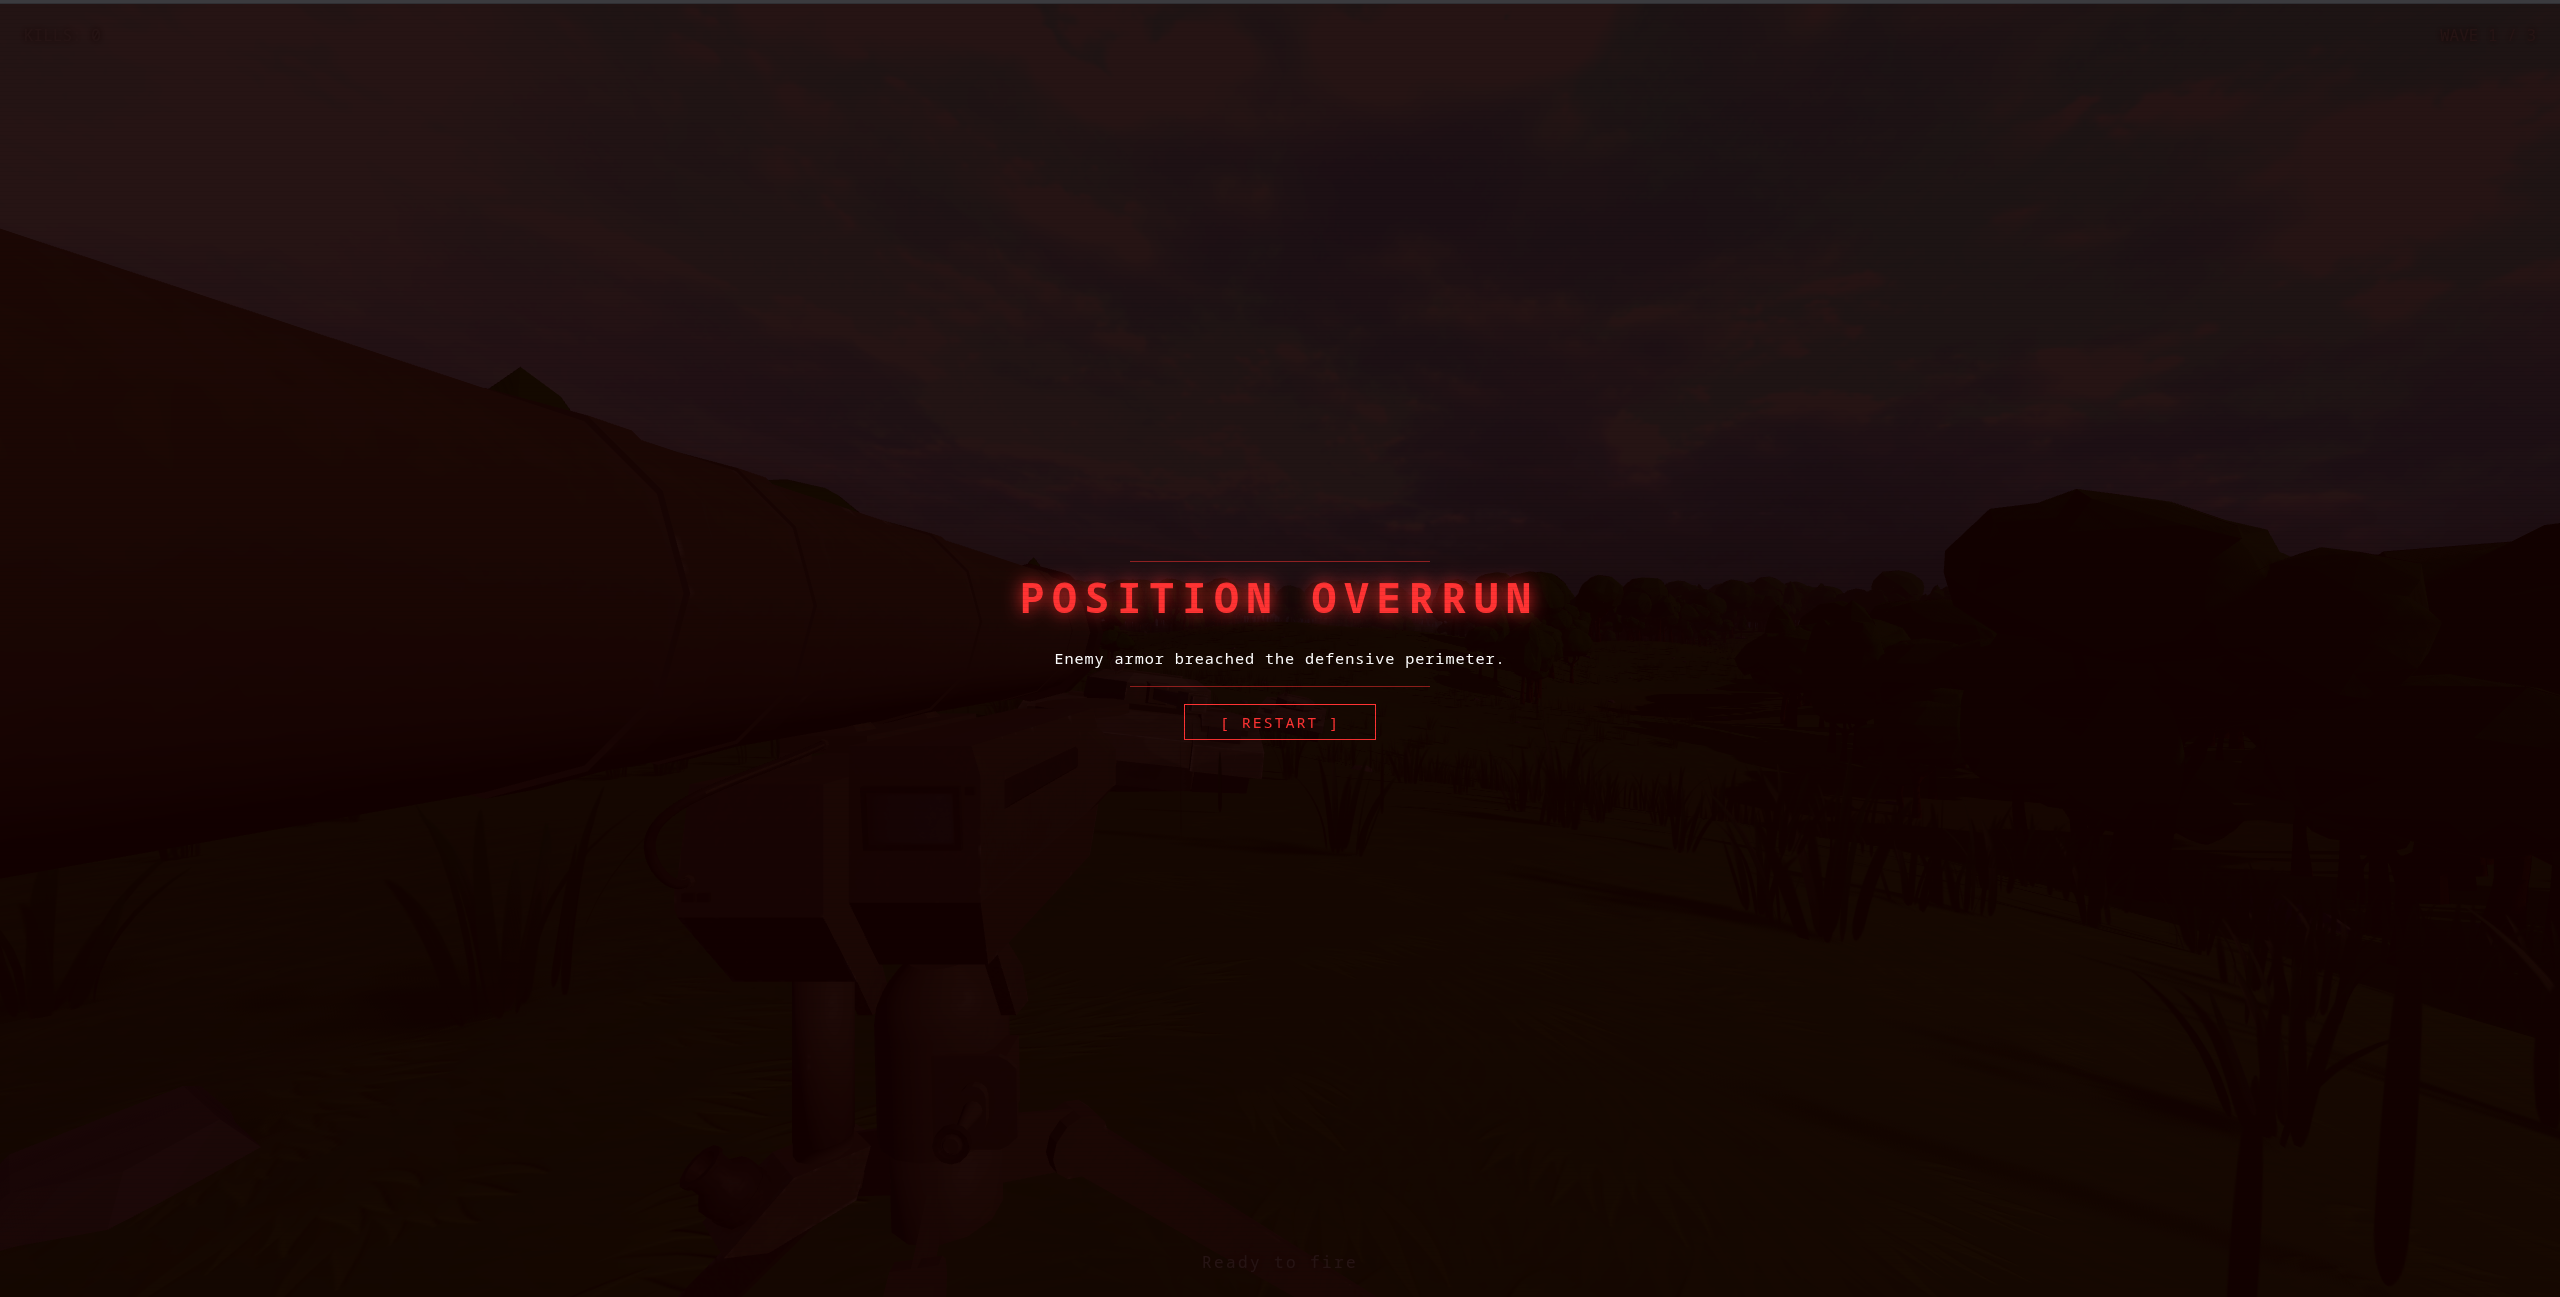
\includegraphics[width=\textwidth]{lose.png}
		\caption{Game Over screen when tanks get too close.}
		\label{fig:loss-screen}
	\end{figure}

	% ════════════════════════════════════════════════════════════
	\section{HUD}

	All HUD elements are plain DOM overlays positioned with \texttt{position:~fixed},
	styled in monospace to match the game's terminal aesthetic:

	\begin{itemize}[itemsep=3pt]
		\item \textbf{Kill counter} (top-left): increments on each tank destroyed.
		\item \textbf{Wave counter} (top-right): shows current wave and total (\texttt{WAVE N / 3}).
		\item \textbf{Launcher state} (bottom center): reflects the current launcher
		      state in plain text: \textit{Ready}, \textit{Missile in flight},
		      \textit{Press R to reload}, or \textit{Reloading}.
		\item \textbf{Crosshair}: an SVG asset, visible only while scoped.
		\item \textbf{Wave announcements}: center-screen text, auto-dismissed after 2 seconds.
	\end{itemize}

	% ════════════════════════════════════════════════════════════
	\section{Debug Scenes}
	
	\begin{figure}[h]
		\centering
		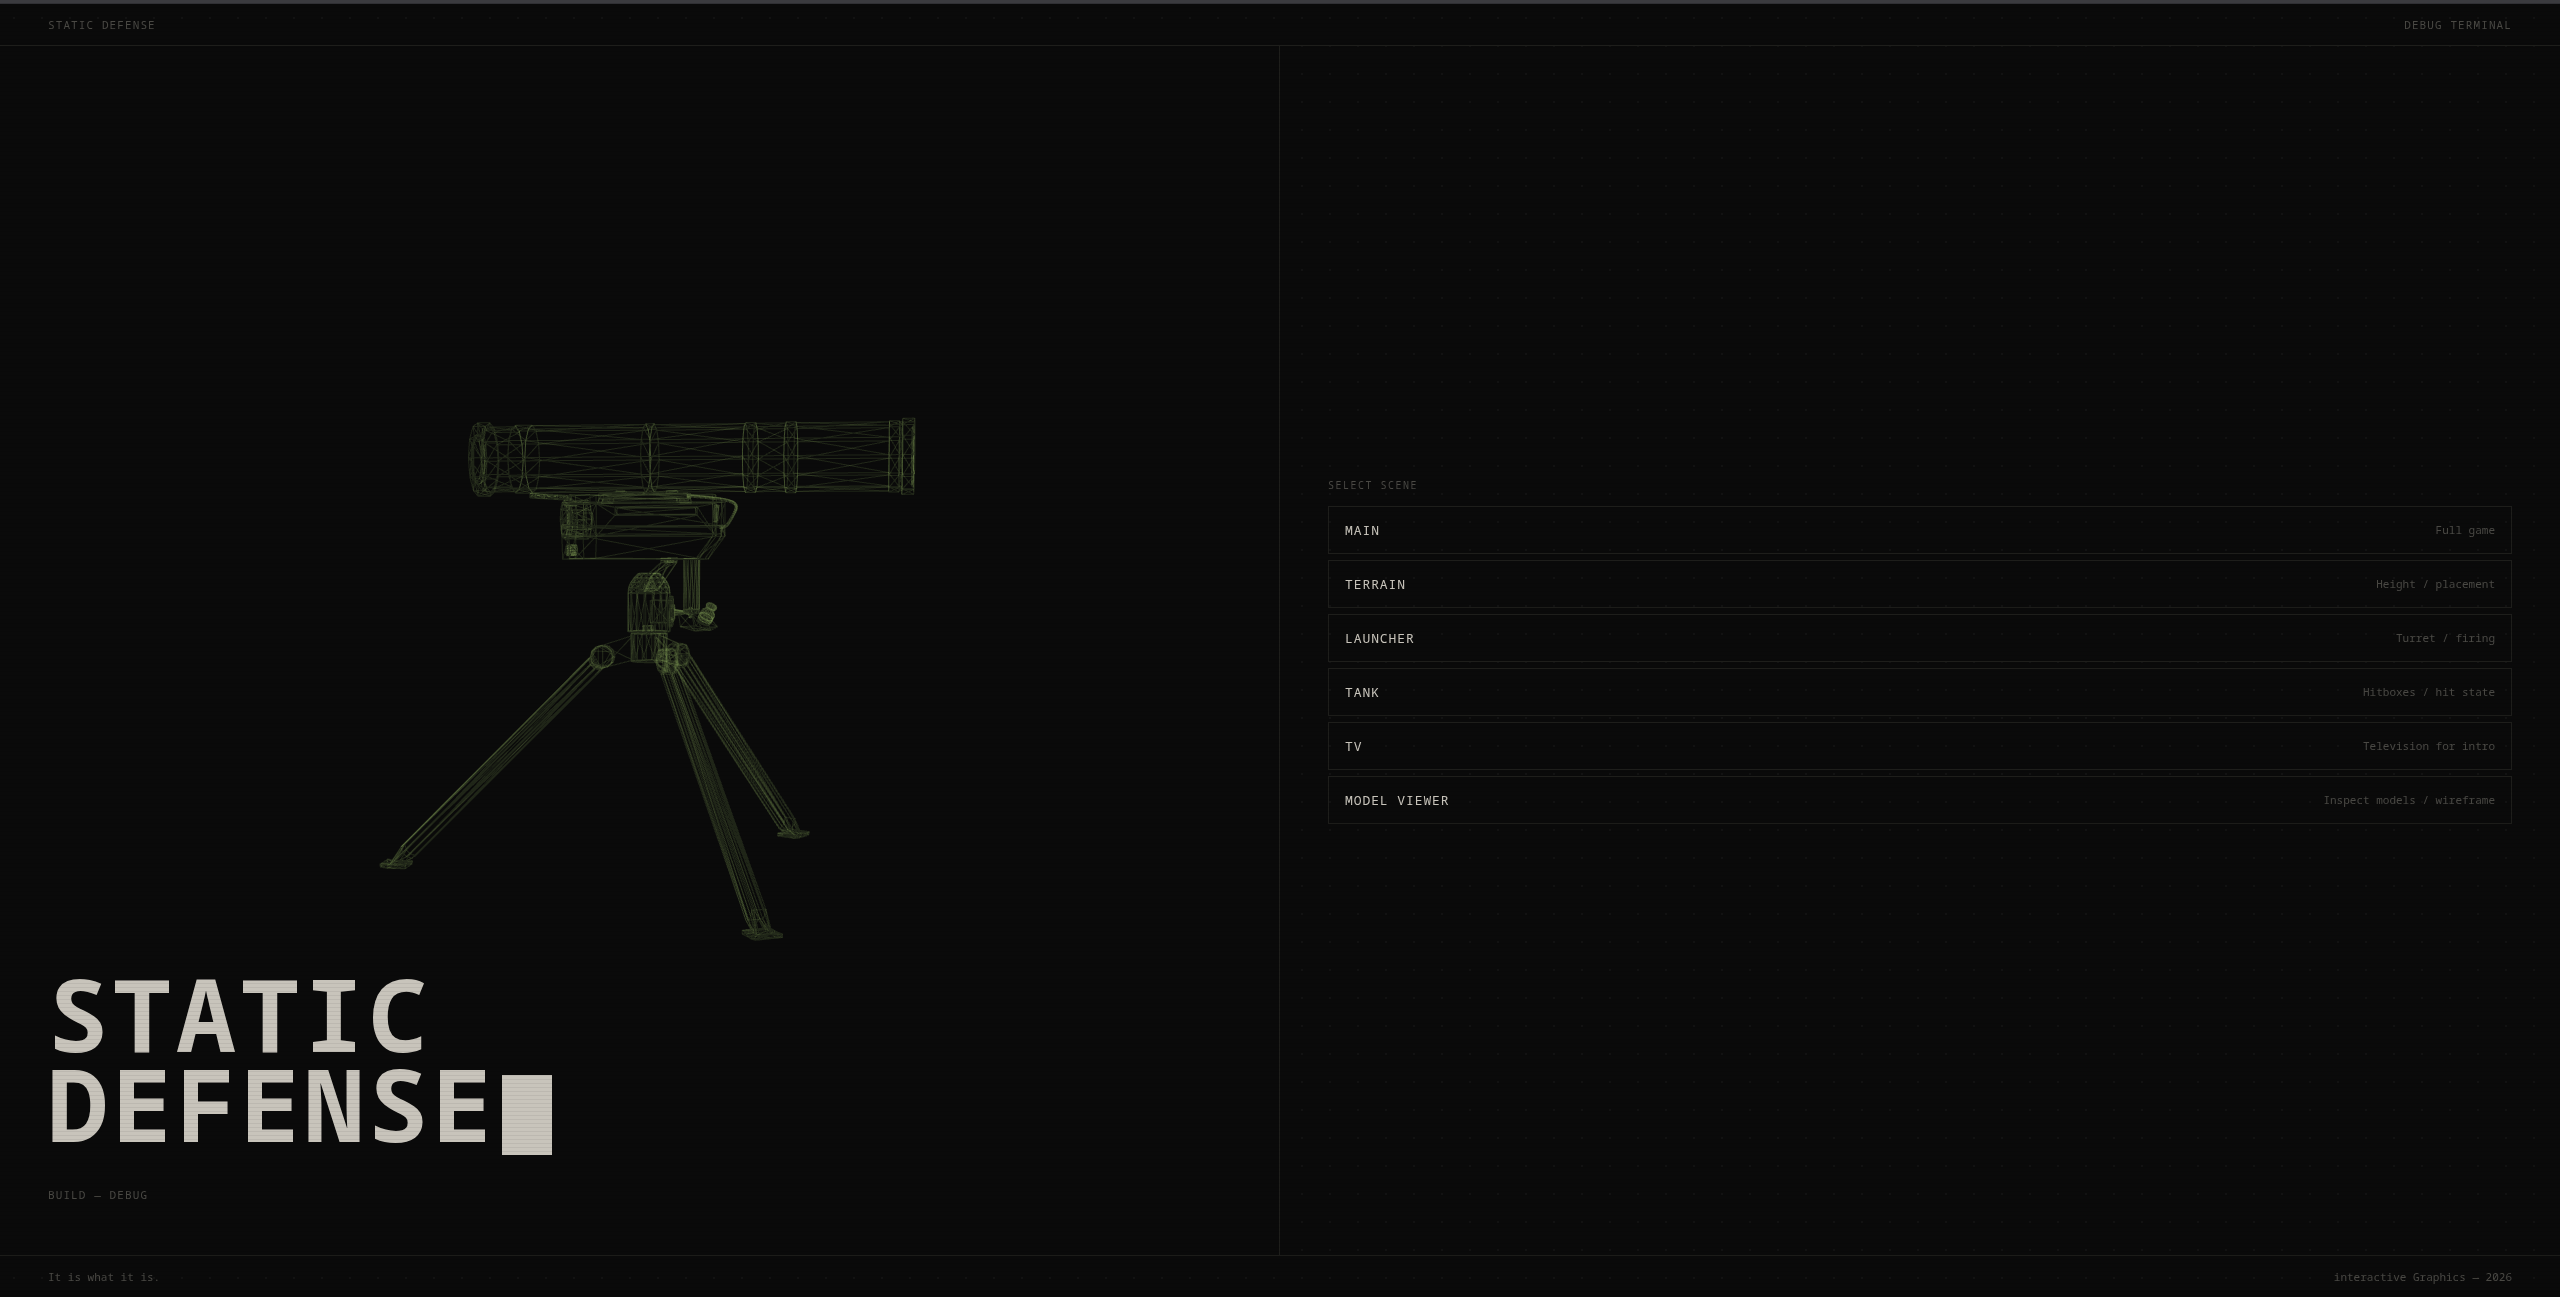
\includegraphics[width=\textwidth]{menu.png}
		\caption{Main menu that allows to select a scene.}
		\label{fig:Main menu}
	\end{figure}

	A URL-parameter-driven scene selector (\texttt{?scene=X}) loads isolated debug
	environments without touching the main game. Five debug scenes are available:

	\begin{itemize}[itemsep=3pt]
		\item \textbf{terrain}: live sliders for size, frequency, amplitude, tree density,
		      grass density, and rock counts. A navmap color overlay (green/red per cell)
		      can be toggled on or off independently of terrain regeneration.
		\item \textbf{launcher}: isolated launcher with full fire and reload, six tanks
		      at staggered distances for missile range calibration.
		\item \textbf{tank}: single tank patrolling toward a fixed target, for state
		      machine and terrain-conforming inspection.
		\item \textbf{tv}: the intro TV prop with video playback in isolation.
		\item \textbf{model}: orbit viewer for all game assets. A sidebar lists every
		      model; clicking or using arrow keys switches the active model. Launcher and
		      tank load their shared in-game PBR materials. \texttt{W} toggles wireframe;
		      \texttt{F} reframes the camera to the model bounding box.
	\end{itemize}

	% ════════════════════════════════════════════════════════════
	\section{Known Limitations}

	\begin{itemize}[itemsep=3pt]
		\item The A* grid is computed once at startup. Wrecked tanks block their cell
		      permanently; active tanks must route around them using their next stuck-detection
		      repath rather than reacting immediately.
		\item The scope vignette and noise canvas are CSS-only overlays and do not
		      integrate with the WebGL depth buffer.
	\end{itemize}

	% ════════════════════════════════════════════════════════════
	\FloatBarrier
	\begin{thebibliography}{9}

		\bibitem{threejs}
		Three.js contributors.
		\textit{Three.js Documentation}.
		Available: \url{https://threejs.org/docs/}. Accessed June 2026.

		\bibitem{vite}
		Evan You et al.
		\textit{Vite Documentation}.
		Available: \url{https://vitejs.dev/}. Accessed June 2026.

		\bibitem{simplexnoise}
		Jonas Wagner.
		\textit{simplex-noise.js} (v4.0.3).
		Available: \url{https://github.com/jwagner/simplex-noise.js}. Accessed June 2026.

		\bibitem{polyhaven}
		Poly Haven.
		\textit{Free HDRIs, Textures and 3D Models}.
		Available: \url{https://polyhaven.com/}. Accessed June 2026.

		\bibitem{pixabay}
		Pixabay, freesound\_community.
		\textit{Royalty-free sound effects}.
		Available: \url{https://pixabay.com/}. Accessed June 2026.

		\bibitem{sketchfab-tank}
		Kolos Studios.
		\textit{Low Poly Tank} [3D model, Sketchfab].
		Available: \url{https://sketchfab.com/3d-models/low-poly-tank-308346f4741a48018c93ebe6f8e53905}.
		Accessed June 2026. (Mesh edited and retextured by the author.)

		\bibitem{sketchfab-trees}
		SimplePolygon.
		\textit{Free Simple Lowpoly Trees} [3D models, Sketchfab].
		Available: \url{https://sketchfab.com/3d-models/free-simple-lowpoly-trees-3d-models-852b73cc6827491681ac56431e790746}.
		Accessed June 2026.

		\bibitem{sketchfab-tv}
		mittelwerk.
		\textit{Portable TV Set} [3D model, Sketchfab].
		Available: \url{https://sketchfab.com/3d-models/portable-tv-set-a8e4e31aa9a0439892b0b32a38a0fa3b}.
		Accessed June 2026.

		\bibitem{sketchfab-rocks}
		\textit{Rock Low Poly} [3D model, Sketchfab].
		Available: \url{https://sketchfab.com/3d-models/rock-low-poly-2c88f234671c4aceb6a6449270b168b0}.
		Accessed June 2026.

		\bibitem{sketchfab-grass}
		Nicothin.
		\textit{Stylized Grass} [3D models, Sketchfab].
		Available: \url{https://sketchfab.com/3d-models/stylized-grass-3a5a5c5be677403d9f56e451cd3dd4af}.
		Accessed June 2026.

		\bibitem{freestylized}
		freestylized.com.
		\textit{Grass Terrain Texture (grass\_01)}.
		Available: \url{https://freestylized.com/material/grass_01/}.
		Accessed June 2026.

	\end{thebibliography}

\end{document}